\documentclass[12pt,english]{article}
\usepackage[T1]{fontenc}

\usepackage[latin9]{inputenc}
\usepackage{geometry}
\geometry{verbose,tmargin=1.0in,bmargin=1.0in,lmargin=1.0in,rmargin=1.0in}
\usepackage{amssymb}
\usepackage{babel}
\usepackage{graphicx}
\usepackage{caption}
\usepackage{hyperref}




%\usepackage{biblatex}

%\usepackage[utf8]{inputenc}

\usepackage{amsthm}
\usepackage{amssymb}

\newcommand{\Halmos}{$\blacksquare$}

\usepackage{hyperref}
%\usepackage{cleveref}
\usepackage[capitalise]{cleveref}
\usepackage{xcolor}

\usepackage[normalem]{ulem}

\newtheorem{lemma}{Lemma}
\renewcommand{\thelemma}{\arabic{lemma}}


\newtheorem{theorem}{Theorem}
\renewcommand{\thetheorem}{\arabic{theorem}}

\newtheorem{proposition}{Proposition}
\renewcommand{\theproposition}{\arabic{proposition}}

\newcommand{\argmax}{\mathrm{argmax}}

\Crefname{table}{Table}{Tables}

\crefname{lemma}{Lemma}{Lemmas}
\crefname{theorem}{Theorem}{Theorems}
\crefname{proposition}{Proposition}{Propositions}
%%% OPREuses endnotes
\usepackage{endnotes}
\let\footnote=\endnote
\let\enotesize=\normalsize
\def\notesname{Endnotes}%
\def\makeenmark{\hbox to1.275em{\theenmark.\enskip\hss}}
\def\enoteformat{\rightskip0pt\leftskip0pt\parindent=1.275em
  \leavevmode\llap{\makeenmark}}
  


% Private macros here (check that there is no clash with the style)

% Natbib setup for author-year style
\usepackage{natbib}
 \bibpunct[, ]{(}{)}{,}{a}{}{,}%
 \def\bibfont{\small}%
 \def\bibsep{\smallskipamount}%
 \def\bibhang{24pt}%
 \def\newblock{\ }%
 \def\BIBand{and}%



\newcommand{\w}{w}
\newcommand{\z}{z}
\newcommand{\dimension}{d}

\newcommand{\pfcomment}[1]{{\color{red} PF: #1}}
\newcommand{\pfedit}[1]{{\color{red} #1}}
\newcommand{\pfdelete}[1]{{\color{red} \sout{#1}}}
\newcommand{\stcomment}[1]{{\color{blue} ST: #1}}
\newcommand{\stedit}[1]{{\color{blue} #1}}
\newcommand{\stdelete}[1]{{\color{blue} \sout{#1}}}
\newcommand{\sigmatilde}{\tilde{\sigma}}
\newcommand\numberthis{\addtocounter{equation}{1}\tag{\theequation}}

\newcommand{\theHalgorithm}{\arabic{algorithm}}


\usepackage{algorithm}
\usepackage{algorithmic}
\usepackage{graphicx}
\usepackage{caption}
\usepackage{mathptmx}
\usepackage{amsmath}
\usepackage{amssymb}

\usepackage{subcaption}
\usepackage{breqn}

\usepackage{bibunits}
\defaultbibliographystyle{natbib}
\defaultbibliography{or}

\newcommand{\abbrv}{MLS}
\newcommand{\name}{Most Likely to Succeed}


\date{}
\linespread{1.5}


%%%%%%%%%%%%%%%%
\begin{document}





\title{Effort Allocation and Statistical Inference\\ for Multistart Stochastic Gradient Descent}


\author{Saul Toscano-Palmerin, Peter I. Frazier\\
st684@cornell.edu, pf98@cornell.edu\\
School of Operations Research \& Information Engineering\\
Cornell University, Ithaca, NY 14853\\
}


\maketitle



\begin{abstract} 
Multistart stochastic gradient descent methods are widely used for gradient-based stochastic global optimization.  While these methods are effective relative to other approaches for these challenging problems, they seem to waste computational resources: starts often converge to local optima or stationary points that are the same or worse than those found by other starts, failing to produce useful information.  
We propose a rule for allocating computational effort across starts, \name\ (\abbrv), which uses computation more efficiently by allocating more resources to the most promising starts.  This allocation rule is based on a novel Gaussian-Process-based statistical model (SGD-GP) for a start's limiting objective value.  Unlike previously proposed statistical models, ours agrees with known convergence rates for SGD. 
Numerical results show our approach improves significantly over four benchmarks:
equal and random allocation rules used widely in practice,
and allocation rules based on two statistical models for learning curves from the machine learning literature.
Our approach often recovers a significantly better global solution than the best of these benchmarks 
and achieves bencharks' solution quality with an order of magnitude less computation.
\end{abstract}


\section{INTRODUCTION}
\label{sec:intro}

Stochastic gradient descent (SGD) methods \citep{robbins,sgd:Nemirovski,adam} are widely used algorithms for training machine learning algorithms \citep{cnn_cifar,murphy2012machine} and optimization via simulation \citep{fu2015}.
Unfortunately, when the objective function is non-convex, these methods may converge to a saddle point or local optimum, instead of a global optimum. Furthermore, even when the objective function is convex, SGD may converge slowly to a global optimum when started from a disadvantageous location. 

A common solution to these challenges is multi-start SGD \citep{schoen:1991,marti:2016}, in which several starting points are chosen uniformly at random, and an SGD algorithm is operated separately starting from each.
(We use the term ``start'' to refer both to an individual starting point, and to the path of SGD starting from an individual point.)
If the number of starts is large enough relative to the number of local optima in the problem, and their starting positions are sufficiently diverse, multi-start SGD is likely to find a global optimum.  

Multi-start SGD, however, often seems to waste computation.  Several starts may converge to the same local optimum, providing essentially the same information about that local optimum's location and value as a single start among them, but consuming several-fold more computation. Also, starts converging to local optima or stationary points worse than an incumbent contribute little to the final solution.
While simply reducing the number of starts risks failing to find the global optimum, intuition suggests that substantial computational savings might be achieved by intelligently allocating computational effort across starts: if a start seems unlikely to provide a new globally optimal solution, then we can compute fewer additional iterations and instead allocate more computational effort toward the most promising starts.


%\paragraph{Contributions:}
In this paper, we make two contributions. The first is a rule for sequentially allocating computational effort across starts, called ``\name'' (\abbrv).  This allocation rule is built on a Bayesian statistical model for the limiting value of the objective function along SGD's path from a single start.  It chooses to allocate effort to the start that is most likely (according to this statistical model) to provide an objective value at convergence that exceeds an incumbent best solution.

% Our policy depends on building a Bayesian model on the value of the objective function at convergence of each starting point, which depends on a non-stationary Gaussian process \cite{RaWi06}. 
% Our \name policy chooses to move one step in a SGD curve of a particular starting point if the posterior probability of its convergent value of being better than the current best observed value is larger than the respective posterior probability of any other starting point. The previous probabilities are computed using our SGD-GP model.

The second contribution is this statistical model, which we call SGD-GP.  Using the iterates $x_1,\ldots,x_n$ from one start of SGD, this statistical model calculates a posterior probability distribution on the value of the objective at the limit of the iterate sequence, $f(x_\infty)$, and on the scaled distance between the current iterate and this limit, $\sqrt{n}(x_n - x_\infty)$.
This statistical model is derived from asymptotic theory for stochastic gradient descent \citep{kushner}, which shows 
that $\sqrt{n}(x_{n}-x_{\infty})$ behaves asymptotically like an Ornstein-Uhlenbeck process under some conditions.
This use of the asymptotic theory stands in contrast to existing approaches for modeling paths from SGD, discussed in more detail below. In some cases these existing approaches assume exponential rates of convergence while SGD does not converge exponentially fast, and none to our knowledge have been shown to be compatible with SGD's known asymptotic behavior.


We demonstrate that \abbrv\ together with SGD-GP substantially outperforms the best of four benchmarks:
Equal Allocation;
Random Allocation;
and two statistical models for learning curves from the machine learning literature \citep{Swersky:2014,Hutter:2015}
together with the MLS allocation rule.
While equal and random allocation are often considered weak benchmarks in the ranking and selection literature \citep{kim:20062}, they are more meaningful here because no other methods have been proposed for allocating effort in SGD 
to our knowledge,
making them the state of the art.  (\cite{Swersky:2014,Hutter:2015} considered other application settings, and their allocation rules do not apply directly to the setting we consider here.)
Our approach often recovers a significantly better global solution than the best of these benchmarks 
and achieves bencharks' solution quality with an order of magnitude less computation. We also provide an implementation of both \abbrv\ and SGD-GP on github \citep{MLS}.

Our numerical experiments use the 20-dimensional Rosenbrock function, and three one-\\dimensional objective functions: a concave function (we maximize rather than minimize), a multi-modal function, and an objective whose gradient is nearly zero over a substantial part of the interval.  This last problem is intended to replicate problems with many stationary points, as is believed to arise when training the weights of neural networks \citep{yoshua94}.
Our 20-dimensional problem uses noisy observations of both gradients and the objective, while our one-dimensional problems assume that objective function observations are noise-free. 

This journal paper extends a previous conference paper, \cite{multi_start}. Here, we remove two severe restrictions in that conference paper: one-dimensional inputs and noise-free observations of the objective function.  While we build on the version of SGD-GP proposed in that conference paper, handling multiple dimensions and noisy objective function observations requires substantial additional innovation.  Removing these restrictions makes our method relevant in practical problems.
% PF: I'm going to comment this out for now, until we actually demonstrate this.
% , including training machine learning algorithms such as neural networks that usually have millions of parameters.
The current journal version also adds new experiments and clarifies exposition.


\paragraph{Related Work:}
Previously \cite{boender:1987} developed Bayesian procedures for choosing the number of starts, assuming equal allocation of effort across starts.
This procedure is based on a posterior distribution on the number of local optima, and uses a stopping rule that trades the computational cost of adding more starts against the increased risk of failing to include a start that converges to the globally optimal local optimum. More recently, \cite{frazier2009calibration} developed a statistical model for the path generated by an SGD-based approximate dynamic programming algorithm (it assumed an exponential convergence rate), and \cite{chen2016} presents a method to estimate confidence intervals for the limit of an SGD iterate sequence.


Related work also appears in machine learning, on modeling learning curves \citep{Swersky:2014,Hutter:2015,klein2016fast,boca2017,li2016}. Some of this work studies how loss on a validation dataset changes with the number of iterations in an SGD algorithm  \citep{Swersky:2014,Hutter:2015} and the amount of training data used  \citep{klein2016fast}. 
Some of this work   \citep{Hutter:2015} focuses primarily on statistical modeling of the path of a single start from SGD without considering effort allocation.  In other work  \citep{Swersky:2014,klein2016fast}, a statistical model is used by a search procedure to find a set of hyperparameters in a low-dimensional vector space for which the test loss provided by SGD after some fixed finite number of iterations is minimal.  

Of the work on statistical models for the paths of SGD, ours is unique in that it is derived from SGD's asymptotic convergence theory, and matches known convergence rates.  For example, \cite{Swersky:2014} assumes exponential convergence rates.
In addition, \cite{Swersky:2014} and \cite{Hutter:2015} use only observations of $f(x_{n})$ and model $f(x_n)$ directly, while our approach uses observations of $f(x_n)$, $\nabla f(x_n)$, and $x_n$, and models the scaled distance from the optimum $\sqrt{n}(x_{n}-x_{\infty})$ in addition to $f(x_n)$.
Our use of additional information offers an opportunity for improved accuracy.
In addition, \cite{Hutter:2015} proposes a parametric model, while our approach is non-parametric.

Existing work on computational effort allocation from this line of literature differs from our own in that it focuses on choosing an optimal set of hyperpamaters for a machine learning model, where the value of a set of hyperparameters is the value after some fixed amount $T$ of effort used to find an approximate local optimum corresponding to a single start.  In other words, it focuses on solving $\max_z g(x^1_T;z)$, where $z\in\mathbb{R}^d$ indexes sets of hyperparameter, and $g(x^1_T;z)$ is the {\it test} loss for a set of model parameters $x^1_T$ obtained using $T$ iterations of SGD (or a training dataset of size $T$) to minimize the {\it training} loss $f(x;z)$ over $x$ with $z$ held fixed.  In contrast, we focus on solving $\min_{i=1,\ldots,I} f(x^i_\infty)$ where $x^i_\infty$ is the limiting point of a sequence of SGD iterates. 

In addition, \cite{Hutter:2015} differs in that the statistical model is used to terminate paths early, and once a path is terminated it cannot be restarted. \cite{klein2016fast} differs in that the amount of training data (analogous to the number of iterations of SGD) is chosen up-front, and cannot be augmented once evaluation begins. \cite{li2016}  differs in that it is not based on a statistical model, but instead on a simple tournament framework.
The most closely related of these search papers is \cite{Swersky:2014}, which uses the statistical model to ``freeze'' and ``thaw'' paths from SGD associated with different hyperparameters.  This freeze-thaw framework bears similarity to our notion of effort allocation.  Our allocation rule, however, is substantially different, as it is computed from the probability of outperforming some incumbent best solution, while \cite{Swersky:2014} uses an entropy search criterion \citep{entropySearch}.  Our allocation rule is substantially simpler to compute than the entropy search criterion, scales easily to high-dimensions via inherent opportunities for parallelism, and performs better in our numerical experiments.

Our work is also related to the larger literature on Bayesian optimization \citep{jones1998efficient,forrester2008engineering,brochu2010tutorial,frazier2009knowledge}, where a Gaussian process model is used to select points to sample.  Indeed, our \abbrv\ allocation rule is similar in spirit to the probability of improvement acquisition function \citep{brochu2010tutorial}  that arises in that literature. 
 %\pfcomment{If we have space, we can mention the multifidelity literature.}

Our use of a Bayesian statistical model to allocate computational effort across starts resembles allocation rules in ranking and selection \citep{Bechhofer:1995,kim:2007,kim:20062}, especially Bayesian ranking and selection \citep{frazier2009knowledge}, which allocate effort across a finite set of alternatives to find the best one.  These problems differ in that samples in ranking and selection are typically independent and identically distributed, while in our setting samples are correlated and not identically distributed.

The rest of this paper is organized as follows: $\mathsection$\ref{statistical_model} and $\mathsection$\ref{MLS} describe our SGD-GP model and \name\ allocation rule, respectively. $\mathsection$\ref{experiments} presents numerical experiments. $\mathsection$\ref{conclusion} concludes.

\section{THE SGD-GP STATISTICAL MODEL}
\label{statistical_model}

Stochastic gradient descent (SGD) algorithms are used to minimize an objective function $f(x)$ using stochastic gradients, i.e., unbiased estimates of $\nabla f(x)$. SGD iterations are usually of the form
\begin{equation}
X_{n+1}=\Pi_{A}\left[X_{n}+\lambda_{n}Y_{n}\right],\label{eq:SGD}
\end{equation}
where $\Pi_{A}$ is the projection onto some feasible set $A$ (for unconstrained optimization, $A$ can be taken to be the domain of $f$, and the projection effectively dropped),
$\lambda_{n}$ is the learning rate at iteration $n$, and $Y_{n}$ is a stochastic gradient of $-f$ at $X_{n}$.  A common choice of the learning rate is given by $\lambda_{n}:=\lambda_{0}/n$, where $\lambda_{0}$ is a chosen parameter, although other more sophisticated rules are also often considered \citep{powell2007approximate}. In this paper, we use  $\lambda_{n}:=1/n$ for simplicity of presentation. (Our approach can be generalized to other stepsize sequences, and discuss one such extension below.)  In addition, we use the term SGD to refer generically to the use of \eqref{eq:SGD} to minimize or maximize a function $f$, rather than using the separate terminology stochastic gradient ascent (SGA) when we maximize (in which case $Y_n$ is a stochastic gradient of $f$, rather than $-f$).  Whether we are maximizing or minimizing will be clear from context.

In this section, we develop a Bayesian statistical model for the scaled distance from optimum $\sqrt{n}\left(X_{n}-X_{\infty}\right)$, which is used to build other Bayesian statistical model of the value of the objective function $f$ at the limiting value of a sequence of SGD iterates, $f(X_\infty)$.  Within our \abbrv\ allocation rule, we will apply this model separately to the sequence of iterates from each start.

We create our statistical model in three steps.  
In the first step ($\mathsection$\ref{sec:SGD-GP-1}),  we construct a Bayesian statistical model over the {\it distance} between the current iterate $X_n$ and the limit point $X_\infty$ \stedit{assuming that the domain of $f$ is one-dimensional}.  This statistical model uses the asymptotic theory of SGD (see the appendix), which shows that $M(n):=\sqrt{n}\left(X_{n}-X_{\infty}\right)$ behaves like an Ornstein-Uhlenbeck process when $n$ is large.
By  taking rescaled differences between iterates, and noting that an O-U process is a Gaussian process, we are able to construct a Gaussian process over these observed differences and $M(n)$. We then calculate the conditional distribution of $M(n)$ by conditioning on the observed differences. \stedit{In the second step, we extend the previous model of $M(n)$ to high-dimensional spaces by applying the previous approach to each dimension independently.} In the third step ($\mathsection$\ref{sec:SGD-GP-2}), we use the posterior on $M(n)$ to infer the posterior distribution on $f(X_\infty)$.  To accomplish this, we use \stedit{Taylor's theorem, and the past observations, possibly noisy, of $f(X_m)$ for $m \leq n$}.

Before proceeding with this development, we briefly discuss generalization to other stepsize sequences. If the step size sequence $\lambda_{n}$ is not $1/n$ but still satisfies $o(\lambda_{n}) = (\lambda_{n}/\lambda_{n+1})^{1/2}-1$, then our definition $M(n):=\sqrt{n}(X_{n}-X_{\infty})$ can be generalized to $M(n):=(X_{n}-X_{\infty})/ \sqrt{\lambda_{n}}$. Similar arguments to the ones given below can be used to build a statistical model of $f(X_\infty)$. These rely on theorem 2.1 of section 10.2.1 of \cite{kushner}, which show this new $M(n)$ behaves like an an Ornstein-Uhlenbeck process when $n$ is large under mild assumptions. More generally, when the limiting behavior of some rescaled version of $X_n - X_\infty$ is understood, we can apply techniques similar to the ones below.

%${\lambda_{n}}$

%  Although we actually consider stochastic gradient ascent, we refer it as SGD in the development of our method because it is more common than SGA in the literature.

% The previous section $\mathsection$\ref{sec:sga} shows that under mild conditions, $M_{n}:=\sqrt{n}\left(x_{n}-x_{\infty}\right)$ behaves like an Ornstein-Uhlenbeck process when $n$ is large, where $x_{n}$ is the $n-$step of the SGD, and $x_{n}$ converges weakly to $x_{\infty}$.  \pfcomment{This is a good summary --- this plus the definition of SGD plus notation is basically all we need from the previous section }

\subsection{Inference Over $M(n)$ in One-Dimension Given Hyperparameter $\theta$}
\label{sec:SGD-GP-1}

\stedit{We first present a statistical model for $M(n)$, which allows inference from data  $x_{1:n}$ when the domain of the function is one-dimensional. We present this model for known hyperparameters in this section and extend it to unknown hyperparameters  and high-dimensional spaces in the next.}

Assuming that $X_{n}$ is one-dimensional, the asymptotic theory of SGD  (see the appendix) implies that 
$M(n)=\sqrt{n}\left(X_{n}-X_{\infty}\right)$ behaves like an Ornstein-Uhlenbeck process when $n$ is large under mild assumptions.
We assume that these mild assumptions hold in the problem studied, and so 
\[
M(\cdot) \mid \theta\sim GP\left(0,\Sigma_{0}\left(\cdot,\cdot; \theta\right)\right),
\]
where $\Sigma_{0}$ is the parametric positive kernel of the Ornstein-Uhlenbeck process, which is $\Sigma_{0}(n,n';\theta):=\sigma^{2}e^{-\theta\left|n-m\right|}$ (the {\it kernel}). 
We additionally place a Bayesian prior distribution $\pi$ on $\theta$ \citep{Neal:GPBayesian}. If we lack a strong prior belief on $\theta$, we may use a flat prior.

We now describe how to compute the posterior distribution on $M(n)$ given $\theta$ and the historical data $X_{1:n}=x_{1:n}$. \stedit{By the following relationship

\[
\sqrt{n}\left(X_{n}-X_{n+1}\right)=M\left(n\right)-\sqrt{\frac{n}{n+1}}M\left(n+1\right),
\]
the conditioning formula for normal random vectors \citep{glasserman:mc} and algebraic manipulations}, this posterior distribution at time $n$ is given by
\[
M\left(n\right)\mid X_{1:n} = x_{1:n},\theta\sim N\left(\mu_{n}\left(n;\theta\right),\Sigma_{n}\left(n,n;\theta\right)\right)
\]
\begin{eqnarray*}
\mu_{n}\left(n;\theta\right)  &=& \gamma_{n}A_{n}^{-1}c_{n}^\intercal\\
\Sigma_{n}\left(n,n;\theta\right) &=&  \Sigma_{0}\left(n,n;\theta\right)-\gamma_{n}A_{n}^{-1}\gamma_{n}^\intercal,
\end{eqnarray*}
% \[
% \mu_{n}\left(n;\theta\right)  = \gamma_{n}A_{n}^{-1} c_{n}^\intercal
% \]
% \[
% \Sigma_{n}\left(n,n;\theta\right) =  \Sigma_{0}\left(n,n;\theta\right)-\gamma_{n}A_{n}^{-1}\gamma_{n}^\intercal,
% \]
where the vectors $\gamma_{n}$ and $c_{n}$ are defined by $\gamma_{n}:=\left(\Sigma_{0}\left(n,1;\theta\right)-\sqrt{\frac{1}{2}}\Sigma_{0}\left(n,2;\theta\right),\ldots,\Sigma_{0}\left(n,n-1;\theta\right)-\sqrt{\frac{n-1}{n}}\Sigma_{0}\left(n,n;\theta\right)\right)$, and
$c_{n}:=\left(x_{1}-x_{2},\ldots,\sqrt{n-1}\left(x_{n-1}-x_{n}\right)\right)$,
%$c_{n}:=\left(\left(x_{1}-x_{2}\right)-\beta_{0}\left(1;\theta\right),\ldots,\sqrt{n-1}\left(x_{n-1}-x_{n}\right)-\beta_{0}\left(n-1;\theta\right)\right)$,
%where $\beta_{0}\left(n;\theta\right):=\mu_{0}\left(n;\theta\right)-\sqrt{\frac{n}{n+1}}\mu_{0}\left(n+1;\theta\right)$, 
and the matrix $A_{n}$ by $A_{n}:=(\Sigma_{0}\left(i,j;\theta\right))_{i,j=1}^{n}$.



\subsection{Inference Over $M(n)$ in Multiple Dimensions, Marginalizing over Hyperparameter $\theta$}
We now extend the statistical model for $M(n)$ from the previous section to handle unknown hyperparameters and high-dimensional $X_{n}$.

We first focus on unknown hyperaparameters in one-dimension. We first show how to compute $p\left(\theta\mid X_{1:n} = x_{1:n}\right)$ where $X_{1}$ is the first point of the SGD algorithm, which allows us to sample $\theta$ from its posterior distribution given $X_{1:n} = x_{1:n}$ via slice sampling \citep{radford2003Slice}. Assuming that $X_{1}=x_{1}$ is given, the density of the posterior distribution of $\theta$ given $X_{1:n} = x_{1:n}$ is
\begin{eqnarray*}
p\left(\theta\mid X_{1:n} = x_{1:n}\right) & \propto & P\left(X_{1:n} = x_{1:n}\mid\theta,X_{1}=x_{1}\right)p\left(\theta\right)\\
 & = & P\left(X_{1}=x_{1},\ldots,X_{n}=x_{n}\mid\theta,X_{1}=x_{1}\right)p\left(\theta\right)\\
 & = & P\left(R\left(n-1\right)=\sqrt{n-1}\left(x_{n-1}-x_{n}\right),\ldots,R\left(1\right)=\left(x_{1}-x_{2}\right)\mid\theta,X_{1}=x_{1}\right)p\left(\theta\right)
\end{eqnarray*}
under the assumption that the prior on $\theta$ is independent of $X_{1}$, and $R(n):= \sqrt{n}\left(X_{n}-X_{n+1}\right)$. In order to compute the previous density, we only need to compute the distribution of the vector $(R(1),\ldots,R(n-1))$ given $\theta$. 

To compute the distribution of $(R(1),\ldots,R(n-1))$, we first observe that 
\[
R(n) = \sqrt{n}\left(X_{n}-X_{n+1}\right) = M\left(n\right)-\sqrt{\frac{n}{n+1}}M\left(n+1\right).
\]
Since $M(n)$ follows a Gaussian process given $\theta$, we then have that
\[
R(\cdot)\mid\theta\sim GP\left(0,\Gamma_{0}\left(\cdot,\cdot;\theta\right)\right)
\]
where 
\begin{eqnarray*}
\Gamma_{0}\left(n,m;\theta\right) & := & \Sigma_{0}\left(n,m;\theta\right)+\sqrt{\frac{n}{n+1}}\sqrt{\frac{m}{m+1}}\Sigma_{0}\left(n+1,m+1;\theta\right)\\
 &  & -\sqrt{\frac{m}{m+1}}\Sigma_{0}\left(n,m+1;\theta\right)-\sqrt{\frac{n}{n+1}}\Sigma_{0}\left(n+1,m;\theta\right).
\end{eqnarray*}
\stcomment{add explanation of the previous computations}

Since we can compute $p\left(\theta\mid X_{1:n} = x_{1:n}\right)$, we can sample $\theta$ from its posterior distribution using slice sampling. 


\stedit{We now extend the previous one-dimensional approach to multiple dimensions. We know that $M(n)=\sqrt{n}\left(X_{n}-X_{\infty}\right)$ behaves like an Ornstein-Uhlenbeck process, which implies that the component of each dimension can be modeled by

\[
M_{i}(\cdot) \mid \theta_{i}\sim GP\left(0,\Sigma_{0}\left(\cdot,\cdot; \theta_{i}\right)\right),
\]

where $M_{i}(\cdot)$ is the $i-th$ entry of $M(\cdot)$, $\Sigma_{0}(n,n';\theta_{i}):=\sigma_{i}^{2}e^{-\theta_{i}\left|n-m\right|}$. We additionally place a Bayesian prior distribution $\pi$ on $(\theta_{1},\ldots,\theta_{d})$ where $d$ is the dimension of the domain of the problem.

Following the same previous arguments, we can do inference over $M_{i}$  marginalizing over hyperparameters $\theta_{i}$, which allows us to do inference over $M$.} \stcomment{add the precise theorem, and say that we assume that Q is diagonal to simplify computations?}

\subsection{Inference Over $f(X_\infty)$}
\label{sec:SGD-GP-2}
We now complete our description of the SGD-GP method for statistical inference by describing how 
it infers an approximate posterior distribution for $f\left(X_{\infty}\right)$ given $X_{1:n} = x_{1:n}$, \stedit{and possibly noisy observations of $f(X_n)=f(x_n)$, and $\nabla f\left(x_{n}\right)$}. It uses \stedit{Taylor's theorem} together with the posterior on $M(n)$ described in the previous section. 




To infer $f(X_\infty)$, we first note that 
Taylor's theorem implies
\begin{equation}
\label{eq:a}
f\left(X_{\infty}\right) \approx f\left(X_{n}\right)+\nabla f\left(X_{n}\right)\left(X_{\infty}-X_{n}\right).
\end{equation}

Thus, we only need to estimate $f\left(X_{n}\right)$ and $\nabla f\left(X_{n}\right)$ since we already have a statistical model for $\left(X_{\infty}-X_{n}\right)$. To support scalable inference in high dimensional spaces, we assume that locally the objective function satisfies:

\[
f\left(x\right)\approx \frac{1}{2}\sum_{i=1}^{d}a_{i}\left(x_{i}-b_{i}\right)^{2}+c.
\]

We update estimates of $a_{i}$, $b_{i}$ and $c$ in a scalable way on the fly. We use the following linear relationship: $\nabla f\left(x\right)_{i}\approx a_{i}(x_{i}-b_{i})$. We then estimate each $a_{i}$ and $b_{i}$ via linear regression on the fly: we maintain exponential moving averages for each dimension of four quantities $\left\{ \bar{h}_{k,i},\bar{x}_{k,i},\bar{x^{2}}_{k,i},\bar{xh}_{k,i}\right\} $ where
$h_{k,i}=\nabla f\left(x_{k}\right)_{i}$. Similarly, we maintain exponential moving averages of $\tilde{f}\left(x_{k}\right)-\frac{1}{2}\sum_{i=1}^{d}a_{i}\left(x_{k,i}-b_{i}\right)^{2}$ to estimate $c$ where $\tilde{f}\left(x_{k}\right)$ is the noisy observation of $f(x_{k})$. \stedit{We can then use the posterior distribution on $M(n)$ together with the previous analysis to obtain a posterior distribution on $f(X_\infty)$.}


%To infer $f(X_\infty)$, we first note that 
%the mean-value theorem implies
%\begin{equation}
%\label{eq:a}
%f\left(X_{\infty}\right)=f\left(X_{n}\right)+L_{n}\left|X_{\infty}-X_{n}\right|
%\end{equation}
%and
%\[
%f\left(X_{\infty}\right)=f\left(X_{n-1}\right)+L_{n-1}\left|X_{\infty}-X_{n-1}\right|,
%\]
%for non-negative numbers $L_{n},L_{n-1}$. When $n$ is large, $L_{n}$ is close to $L_{n-1}$ because $X_{n}$ is close to $X_{n+1}$, and they are both %close to $X_{\infty}$.    Thus we assume that $L_{n}\approx L_{n-1}$, and so
%\begin{eqnarray*}
%f\left(X_{n}\right)-f\left(X_{n-1}\right) & = & L_{n}\left|X_{\infty}-X_{n-1}\right|-L_{n}\left|X_{\infty}-X_{n}\right|\\
% & = & L_{n}\left(\frac{|M\left(n-1\right)|}{\sqrt{n-1}}-\frac{|M\left(n\right)|}{\sqrt{n}}\right). 
%\end{eqnarray*}
%To approximate $L_n$, we use plug-in estimators for $|M(n-1)|$ and $|M(n)|$ equal to their expectation under the posterior, leverage our assumption %that $f(x_n)$ and $f(x_{n-1})$ are observed without noise, where $X_n=x_n$ and $X_{n-1}=x_{n-1}$, and then solve the previous equation for $L_n$ to %obtain the estimator given $\theta$,
%\[
%\hat{L}_{n}\left(\theta\right)=
%\frac{\left|f\left(x_{n}\right)-f\left(x_{n-1}\right)\right|}
%{\left|
%E\left[
%\frac{|M\left(n-1\right)|}{\sqrt{n-1}}
%- \frac{|M\left(n\right)|}{\sqrt{n}}
%\mid X_{1:n} = x_{1:n},\theta
%\right]
%\right|}.
%\]

%We can then use this estimator $\hat{L}_n$ along with \eqref{eq:a} and a noise-free observation of $f(x_n)$ to describe the posterior distribution of $f(x_\infty)$ as,
%\[
%f\left(X_{\infty}\right)\mid x_{1:n} \sim f\left(x_{n}\right)+\frac{1}{\sqrt{n}}Z_{n}
%\]
%where the density of $Z_{n}$ is given by 
% \[
% g\left(z\right)=\int_{\theta}p\left(\theta\mid x_{1:n}\right)\phi\left(\frac{\left(z-\hat{L_{n}}\left(\theta\right)E\left[M\left(n\right)\mid x_{1:n},\theta\right]\right)}{\hat{L_{n}}\left(\theta\right)\sqrt{\mbox{Var}\left[M\left(n\right)\mid x_{1:n},\theta\right]}};\theta\right)d\theta,
% \]
%\[
%g\left(z\right)=\int_{\theta}p\left(\theta\mid x_{1:n}\right)\gamma_{\theta}\left(z\right)d\theta,
%\]
%where $\gamma_{\theta}$ is the density of the absolute value of the conditionally (given $\theta$) normal random variable $\hat{L}_n(\theta) M(n)$. (Here, $\hat{L}_n(\theta)$ is treated as conditionally constant given $\theta$, and $M(n)$ is random.)
%absolute value of a
%normal random variable with mean $\hat{L_{n}}\left(\theta\right)E\left[M\left(n\right)\mid x_{1:n},\theta\right]$
%and variance equal to $\hat{L}_{n}^{2}\left(\theta\right)\mbox{Var}\left[M\left(n\right)\mid x_{1:n},\theta\right]$.

%In the case that $f$ is Lipschitz continuous, and we can know the Lipschitz constant $L$, we can use directly $L$ instead of $\hat{L_{n}}\left(\theta\right)$. However, this method overestimates $f\left(x_{\infty}\right)$, because it assumes that $f\left(x_{\infty}\right)-f\left(x_{n}\right)=L\left\Vert x_{n}-x_{\infty}\right\Vert$, while $L_n$ obtained by the mean-value theorem approaches $0$ as $n$ goes to $\infty$ given continuous differentiability of the objective.

\section{THE MOST LIKELY TO SUCCEED ALLOCATION RULE}
\label{MLS}

% As discussed above, users of multi-start stochastic gradient ascent face a dilemma.

As discussed above, multi-start stochastic gradient ascent can waste computation: typically only the limiting value of the best start is used as the final solution, but a substantial amount of computation is spent computing iterates for other starts.  In this section, we use the statistical model from the previous section for choosing how to allocate computational effort across starts.  The goal is to allocate more effort to starts that are likely to produce good limiting values, so that a final solution of equal quality can be produced with less computational effort. We call this rule for allocating effort \name\ (\abbrv).

To support our definition, we first augment our existing notation, using $X_n^i$ to indicate the $n^{\mathrm{th}}$ iterate of SGD using start $i$.   We let $I$ denote the number of starts.
The starting values of $X^i_1$ may be generated arbitrarily, but we recommend choosing them by sampling uniformly at random from the input space.  Then, $X^i_n$ is given recursively from $X^i_{n-1}$ by \eqref{eq:SGD}.

We consider a situation in which starts are advanced one at a time, with an allocation rule deciding which start to advance to its next iteration in each timestep. \stedit{However, parallel allocation is a natural generalization of the previous scenario.}
We will let $t \in \mathbb{Z}_+$ count the number of iterations that have been performed across all of the starts, and we let $n(t,i)$ count the number of iterations performed for start $i$ by time $t$.
Thus, $X_{n(t,i)}^i$ is the value of start $i$ at time $t$.

Formally, an allocation rule is a sequence of mappings, one for each $t$, from the observable state $H_t := (X^i_m : m \le n(t,i), i \in [I])$ to $[I] = \{1,\ldots,I\}$.  Let $\pi_t$ be the mapping for time $t$, so that $\pi_t(H_t)$ is the start that the allocation rule chooses to advance next at time $t$.  As a result of operating a particular policy, the number of iterations assigned to each start over time, $(n(t,i) : t\ge 0, i \in [I])$ is defined by $n(t+1,i) = n(t,i) + 1\{\pi_t(H_t) = i\}$.

Our \abbrv\ allocation rule uses the previously described SGD-GP statistical model on the value of the limiting objective obtained from each start, $f(X^i_\infty)$. The \abbrv\ allocation rule allocates the next unit of computational effort to the start whose limiting objective value is most likely to be at least $\epsilon>0$ better than the best objective value seen so far.
Formally, this rule is defined as,
\begin{equation*}
\pi_t(H_t) := \argmax_i 
P\left(f\left(X_{\infty}^{i}\right)>Y_t+\epsilon\mid H_{t}\right),
\end{equation*}
where $Y_t$ is the best value of the objective function $f$ \stedit{(or estimated value if the observations are noisy)} seen by time $t$, and $\epsilon$ is a strictly positive number. 

This allocation rule naturally balances exploration and exploitation.  First, it favors allocating effort to those starts that are predicted to have a high value for $f(X_\infty^i)$, thus providing exploitation. 
Second, starts with few iterations will naturally have a great deal of uncertainty about its limiting value.  If we imagine that the posterior distribution on $f(X_{\infty}^{i})$ as approximately normally distributed, and we think of the uncertainty as quantified by the variance under this posterior, then  $P\left(f\left(X_{\infty}^{i}\right)>Y_t+\epsilon\mid H_{t}\right)$ will approach $1/2$ as this uncertainty grows large.   Conversely, another start that has enough iterations to be close to convergence will have only a very small amount of uncertainty, and  $P\left(f\left(X_{\infty}^{i}\right)>Y_t+\epsilon\mid H_{t}\right)$ will approach $0$ for any positive $\epsilon$ as this uncertainty shrinks to $0$. 
This suggests that all starts, even those with a value for $f(X_\infty^i)$ predicted to be poor, do get advanced forward eventually, and that we explore as well as exploit.

Although we do not offer a proof here, we conjecture that these ideas can be used to show that all starts are advanced infinitely often with probability $1$ under \abbrv, and that this in turn employs that \abbrv\ allocation rule provides an asymptotically consistent estimator of $\max_i f(X_\infty^i)$.
We also conjecture that the parameter $\epsilon$ can be used to trade off exploration vs. exploitation, with larger values of $\epsilon$ leading to more effort allocated to starts with substantial uncertainty, and smaller values to more exploitation. However, in our numerical experiments we simply set $\epsilon=0.1$.


%\stedit{\paragraph{Procedure to relax the assumption of observing the objective function without noise.} In this framework, we assume that we can obtain noisy evaluations of $f$. We denote a noisy evaluation of $f$ at $x$ by $\hat{f}(x)$, and we assume that there exists a known $L\in\mathbb{N}$ such that $f(x)\approx q\left(x\right):=\frac{1}{L}\sum_{j=1}^{L}\hat{f}\left(x\right)$ for all $x$. To support the definition of the procedure, we use $x_{-1}^{i}$ to denote the last iterate of SGD using start $i$. We use the following procedure:

%We describe this batching strategy in detail here: 
%\begin{enumerate}
%\item Choose a batch size $B$ and a number of replications $L$. 
%\item Run $B$ iterations of SGD for each start $i\in I$.
%\item For each $i\in I$, let $\hat{f_t^i}$ be an estimate of $f$ at $X_{n(t,i)}^{i}$ obtained by averaging $L$ independent replications.
%\item While budget remains:
%\begin{enumerate}
%\item Choose a starting point $i$ using the  \abbrv\ allocation rule, where $f(X_t^i)$ is replaced by $\hat{f_t^i}$.
%\item Run $B$ iterations of SGD for start $i$.
%\item Let $n(t+B,i) = n(t,i)+B$, $n(t+B,j)=n(t,j)$ for $j\ne i$.
%\item Let $t = t+B$.
%\item Let $\hat{f_t^i}$ be an estimate of $f$ at $X_{n(t,i)}^{i}$ obtained by averaging $L$ independent replications.
%\end{enumerate}
%\end{enumerate}

%We believe that the previous method provides an asymptotically consistent estimator of $\max_i f(x_\infty^i)$ by a similar argument than the one given above.}



\section{NUMERICAL EXPERIMENTS}
\label{experiments}

In this section we present numerical experiments exploring the accuracy and coverage of our statistical approach, and the efficiency of our allocation rule in maximizing functions using multi-start stochastic gradient ascent. In the literature on ranking and selection, the equal allocation (EA) rule is considered a weak benchmark algorithm, because many other more sophisticated allocation rules have been developed. However, in our problem no allocation rules have been developed to the best knowledge of the authors of this article.

We compare our \abbrv\ allocation rule ($\mathsection$\ref{MLS}) against four allocations rules. First we compare with an equal allocation (EA) rule in which each starting point is chosen the same number of times in round-robin fashion.  Formally, this rule is  $\pi_t(H_t) =  n\ \mbox{mod}\ I$. \stedit{Second, we compare against a random allocation rule in which each starting point is chosen at random.} Third, we compare against the statistical model defined in \cite{Swersky:2014} used with the MLS allocation rule.  This rule differs from MLS in its statistical model alone.
Fourth, we tried to use the statistical model defined in \cite{Hutter:2015}. However, the model did not work well, because it is necessary to manually tune many hyperparameters of the model to adapt it to a particular optimization problem, and so we do not include these results so as to focus attention on competitive benchmarks. Experiments demonstrate \abbrv\ significantly outperforms these benchmarks on one-dimensional problems in which we observe objective function values without noise and gradients with noise\stedit{, and on a 20-dimensional problem with noisy evaluations of both the objective function and gradient.} We compare on the following maximization problems: a concave maximization problem ($\mathsection$\ref{concave}), a maximization problem with many local maxima ($\mathsection$\ref{local_maximum}), a maximization problem where the gradient is almost zero in some complete intervals of the domain ($\mathsection$\ref{gradient_vanishing}), \stedit{and a maximization problem of the 20-dimensional Rosenbrock function ($\mathsection$\ref{rosenbrock})}. 

\subsection{A Concave Objective Function}
\label{concave}

Here we compare \abbrv\ and EA on a concave maximization problem $\max_{x} f(x):= \max_{x} -0.5x^2$ 
(Figure~\ref{fig:quadratic}.a) where the stochastic gradient is equal to the true gradient plus standard normal noise.  All starting points converge to the same point in this problem. 

Figure~\ref{fig:quadratic} pictures the results using $9$ starting points. Figure~\ref{fig:quadratic}.c shows that \abbrv\ identifies a solution essentially indistinguishable from the optimal in 15 iterations, while EA takes more than 40 iterations, to find a comparable solution. This is a roughly 3-fold improvement. Figure~\ref{fig:quadratic}.b shows that our statistical model predicts with very high precision a start's limiting objective value after only 10 iterations. 

\begin{figure}[htbp]
\begin{center}
\subcaptionbox{Objective function \\ $f(x):=-0.5x^2$}[0.32\linewidth]{
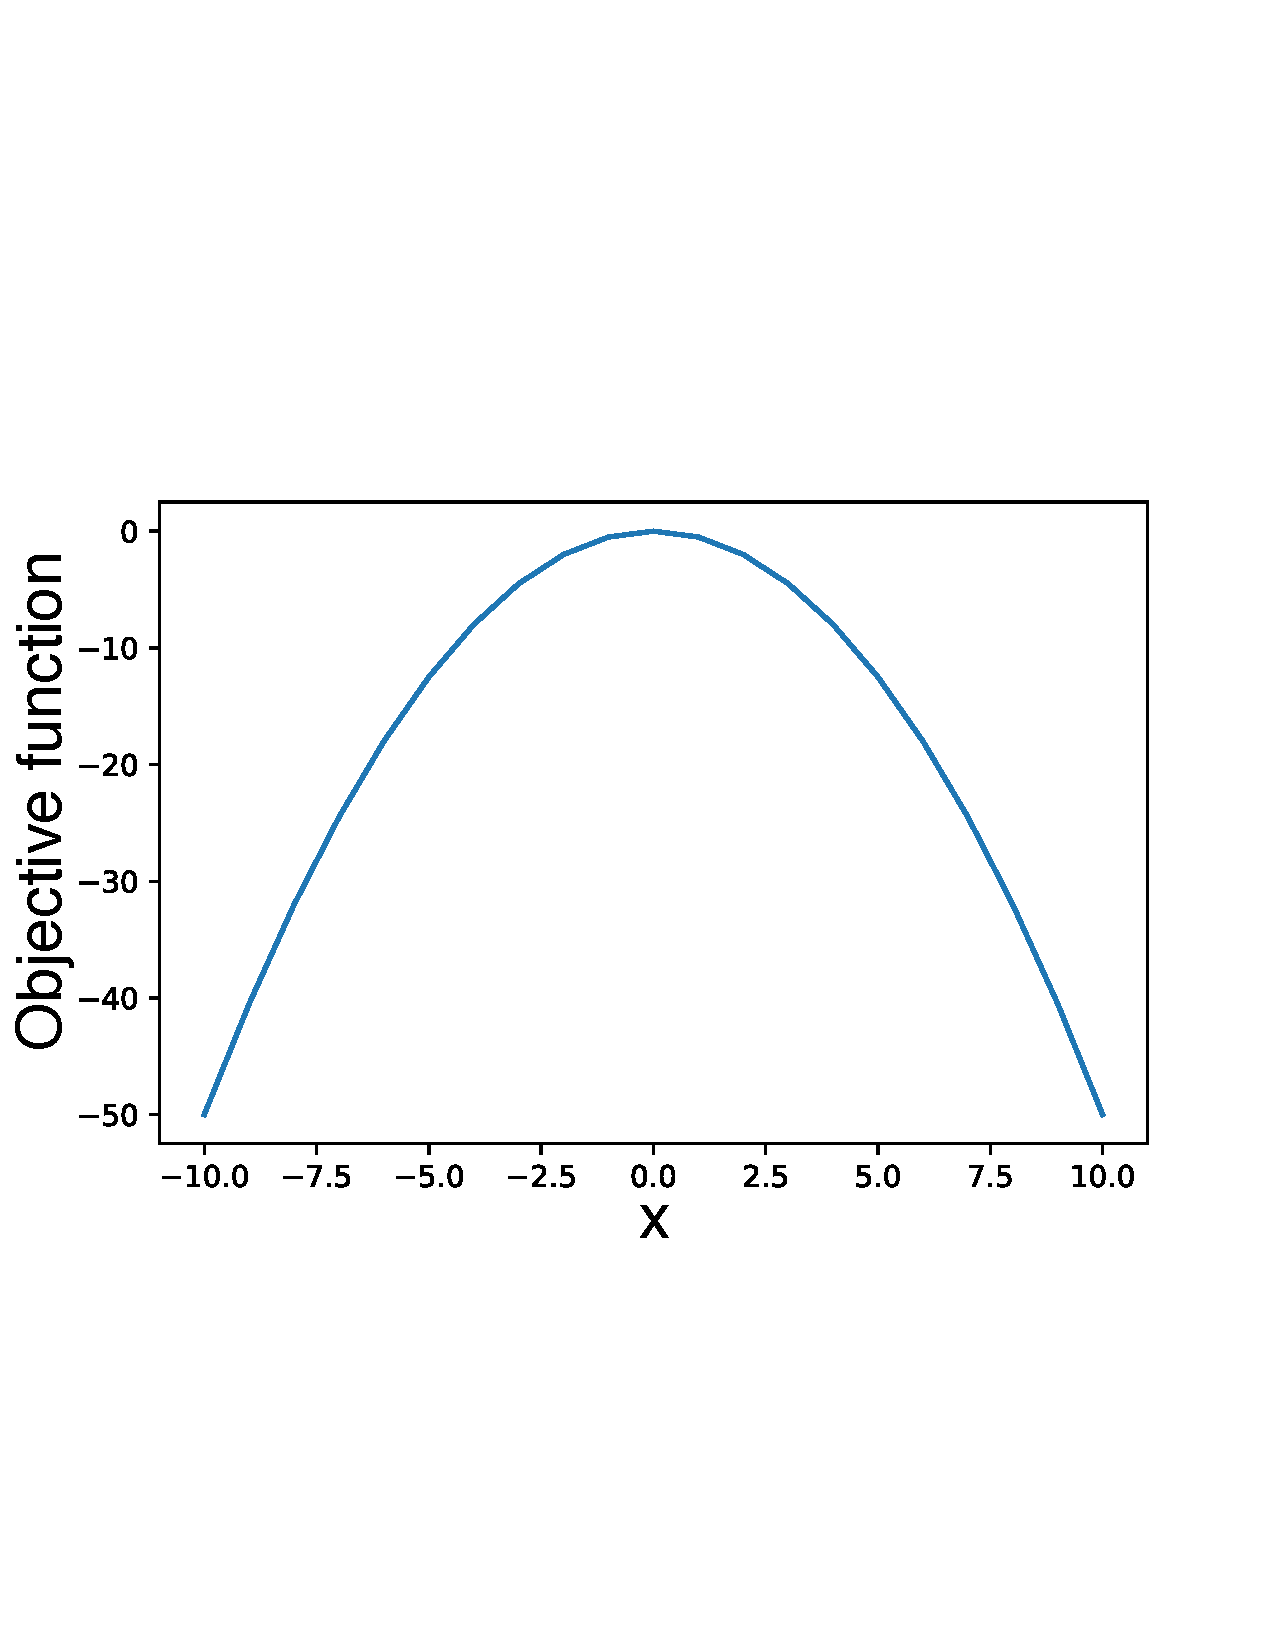
\includegraphics[width=0.32\linewidth,height=2.1in]{plot_quadratic.pdf}}
%   \quad
\subcaptionbox{
SGD-GP's predictions and confidence intervals for the limiting value of SGD ($0$) from a single start.}[0.32\linewidth]{
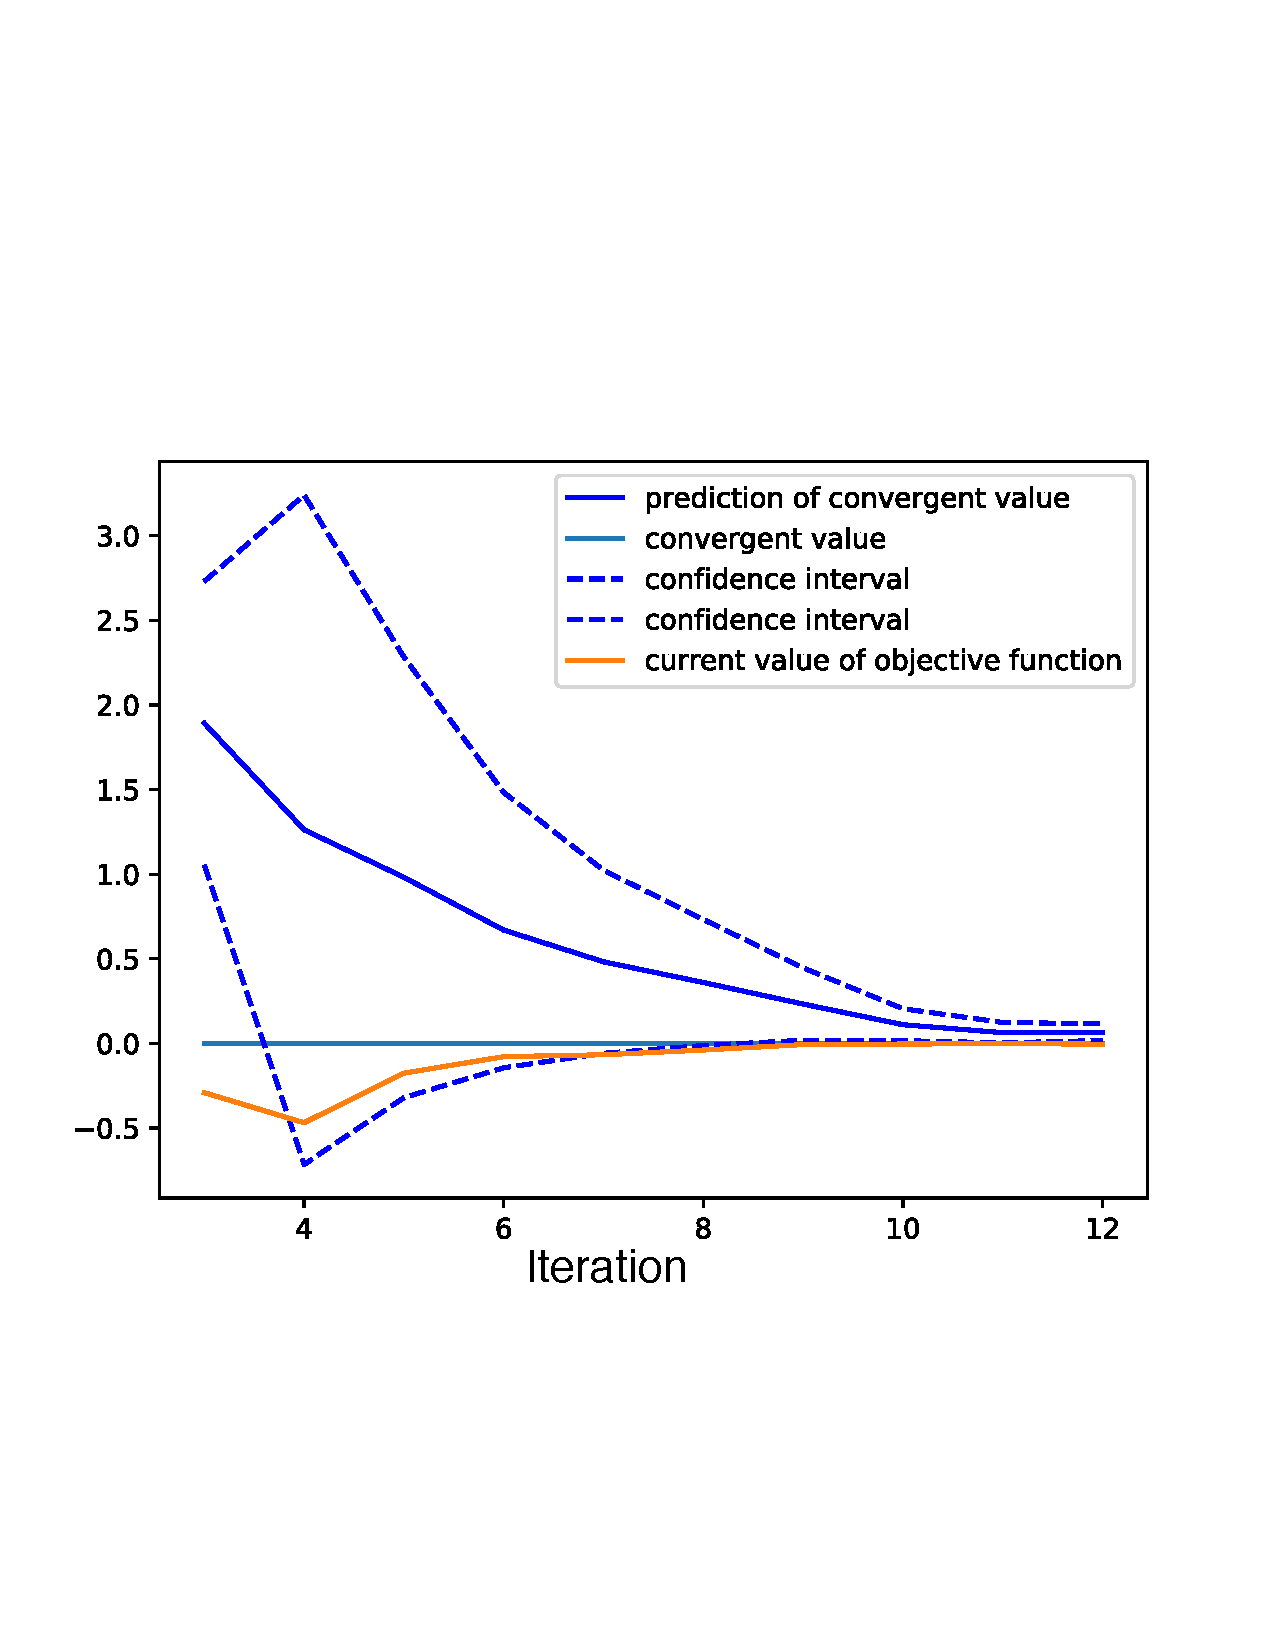
\includegraphics[width=0.32\linewidth,height=2.1in]{quadratic_stat_approx_lipschitz.pdf}}
\quad
\subcaptionbox{
Performance comparison between the \abbrv\ and equal allocation rules using $9$ starting points. 
}[0.32\linewidth]{
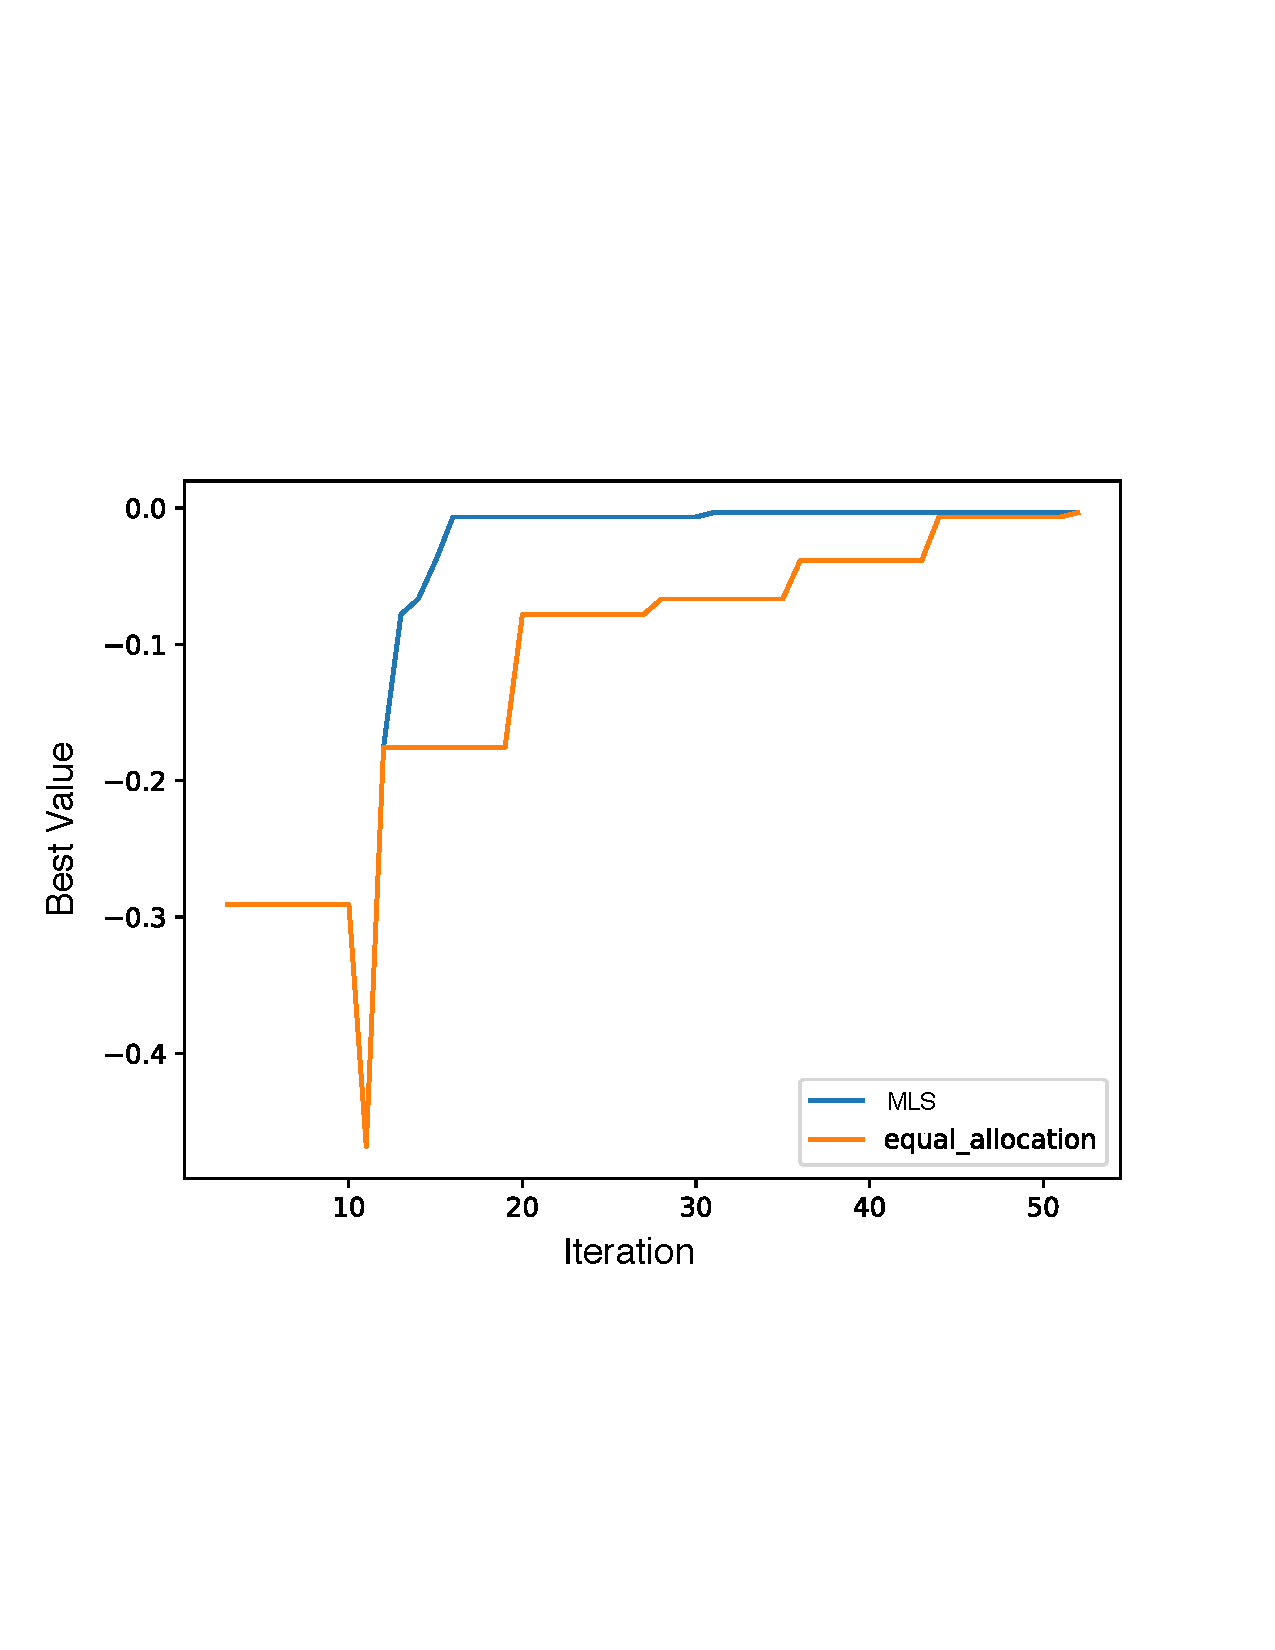
\includegraphics[width=0.32\linewidth,height=2.0in]{greedy_uniform_quadratic.pdf}
}
\smallskip
\caption{
The SGD-GP statistical model (b) and \abbrv\ allocation rule (c) on the problem (a) from $\mathsection$\ref{concave}. (b) shows that SGD-GP can predict the start's limiting objective value with high precision after 10 iterations. (c) shows that our policy finds the optimal solution faster than the equal allocation policy.
\label{fig:quadratic}}
\end{center}
\end{figure}


\subsection{An Objective Function with Many Local Maxima}
\label{local_maximum}
Here we consider an objective function with many local maxima, $f(x):=(1.4-3x)\sin{18x}$, with a domain of $[0,1.2]$. The stochastic gradient is equal to the true gradient plus standard normal noise.
Figure~\ref{fig:multiple_maxima} compares the performance of the \abbrv\ and EA allocation rules with $20$ starting points, plotting the number of iterations beyond the first stage on the $x$ axis, and the average maximum solution. We average over 1200 independent runs of \abbrv\, equal allocation, and Swersky's statistical model with the MLS allocation rule. Our allocation rule identifies the optimal solution much faster than these other rules.

\stedit{Figure~\ref{fig:multiple_maxima}.c shows that \abbrv\ performs much better than the other policies considered. Our policy performs better than the other policies after only 20 iterations. In fact, after 10 iterations, \abbrv\ finds a solution that is comparable to the solution found by the other allocation rules after 100 iterations. This is a roughly 10-fold improvement. Moreover, Figure~\ref{fig:multiple_maxima}.b shows that our statistical model predicts with very high precision a start's limiting objective value after 20 iterations.}

%\clearpage

\begin{figure}[htbp]
\begin{center}
\subcaptionbox{Objective function \\ $f(x):=(1.4-3x)\sin{18x}$}[0.32\linewidth]{
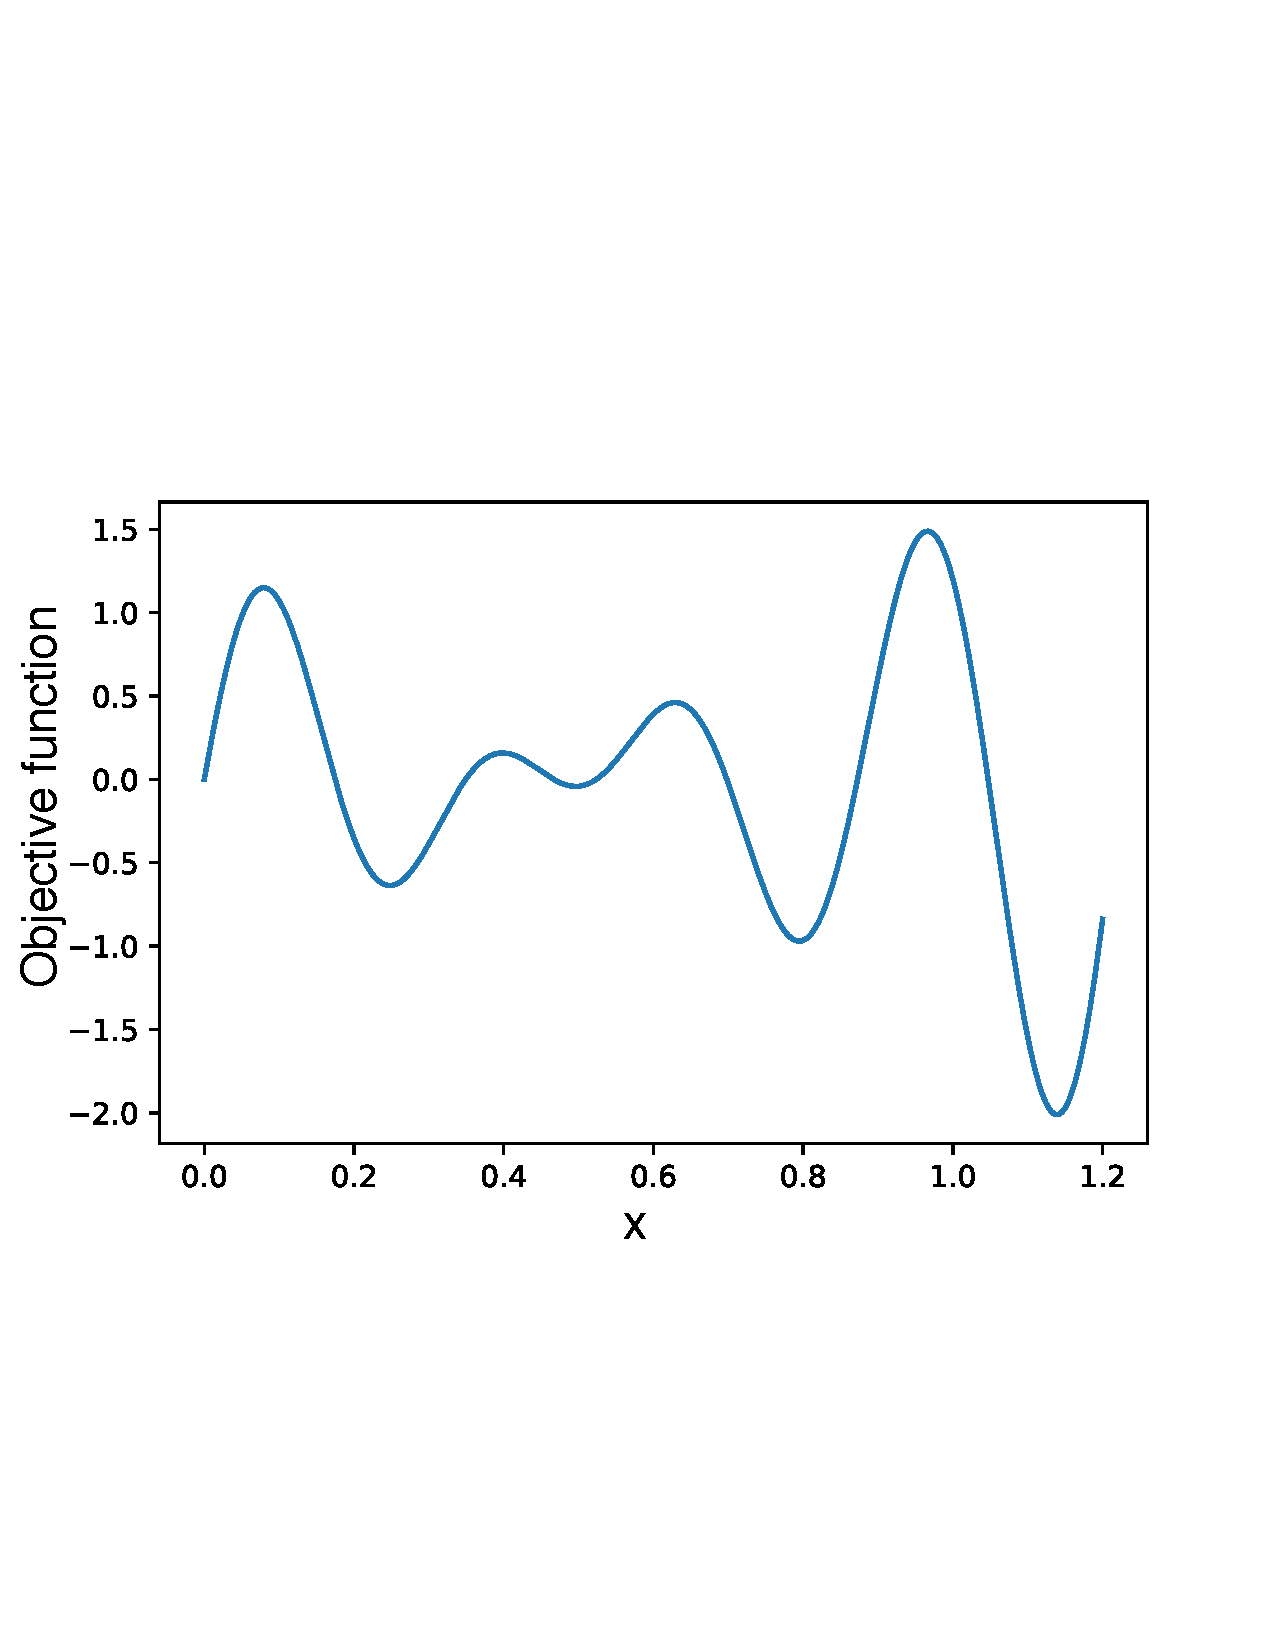
\includegraphics[width=0.32\linewidth,height=2.1in]{plot_problem5.pdf}}
%   \quad
\subcaptionbox{
SGD-GP's predictions and confidence intervals for the limiting value of SGD ($1.49$) from a single start.
}[0.32\linewidth]{
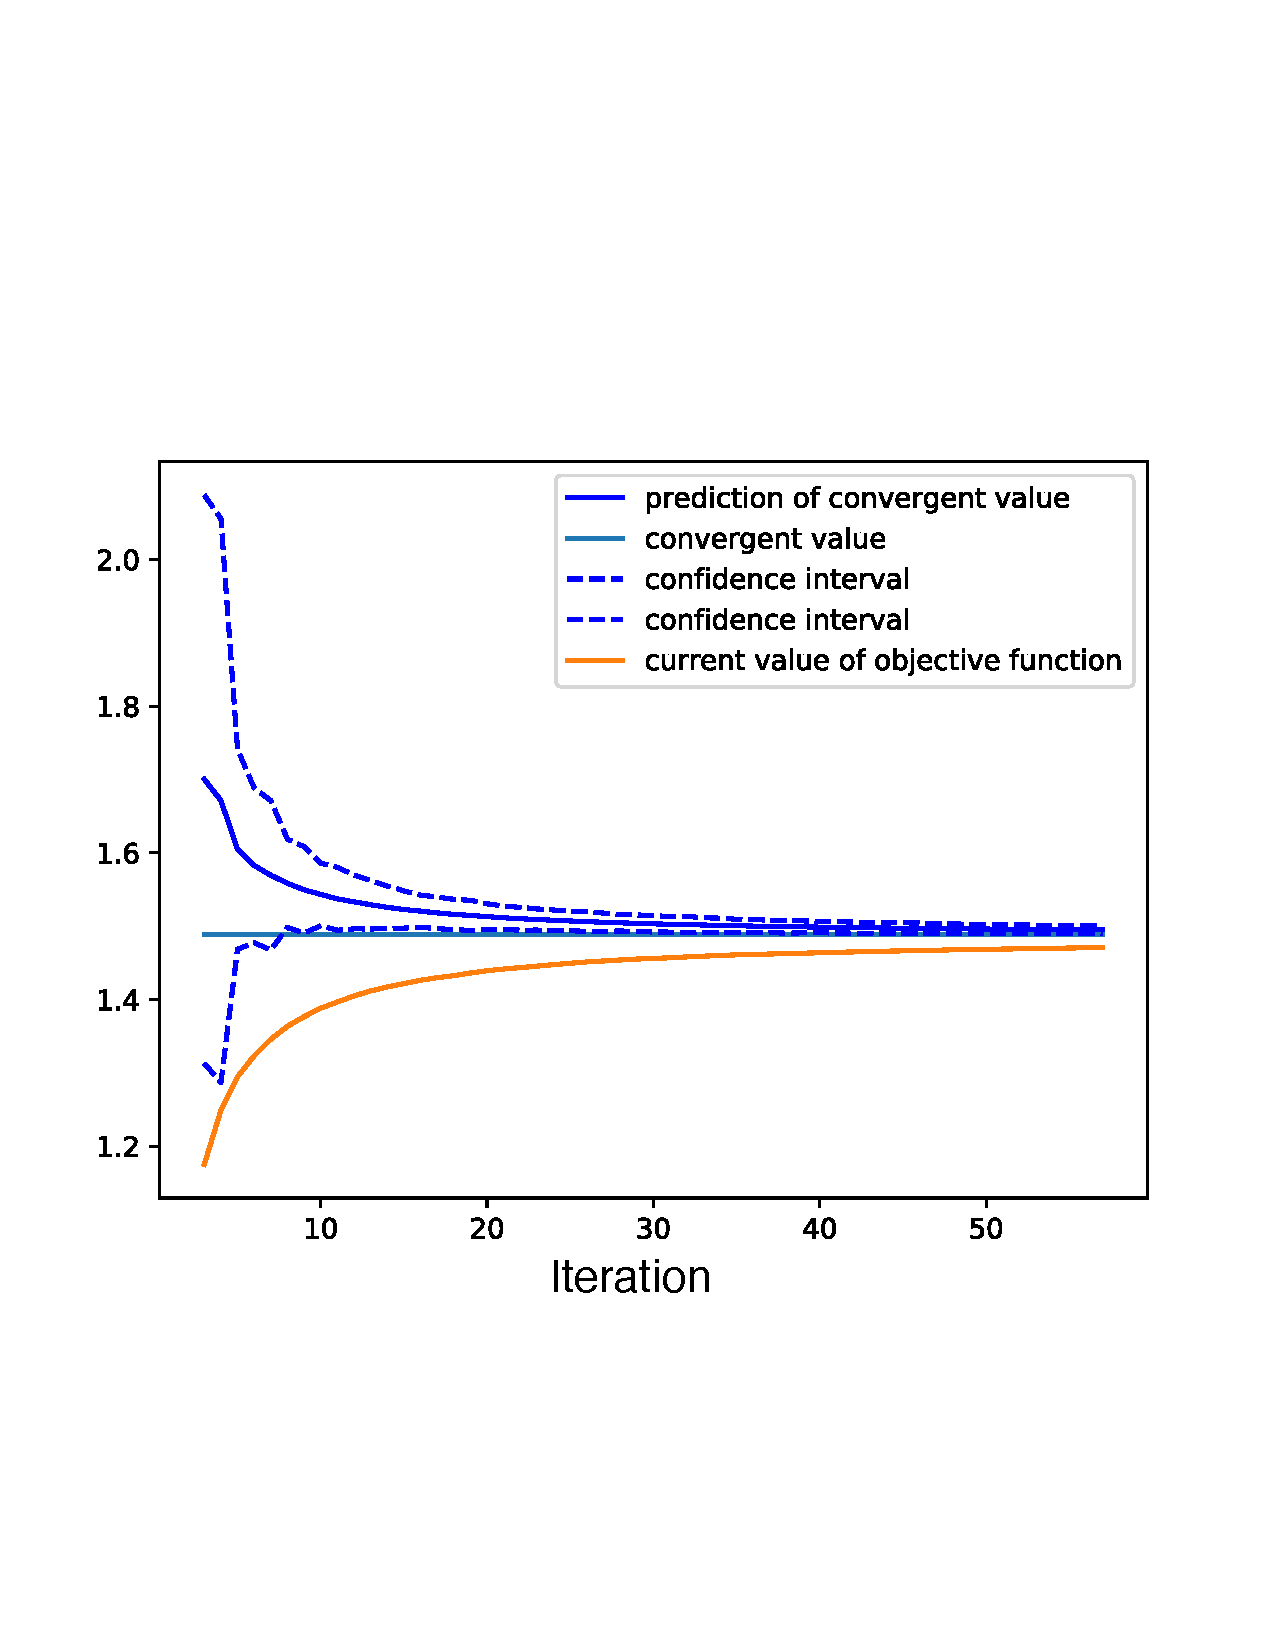
\includegraphics[width=0.32\linewidth,height=2.1in]{stat_model_problem5.pdf}}
\quad
\subcaptionbox{
Performance comparison between \abbrv\, equal allocation, and Swersky's statistical model with the \abbrv\ rule using $20$ starting points.
}[0.32\linewidth]{
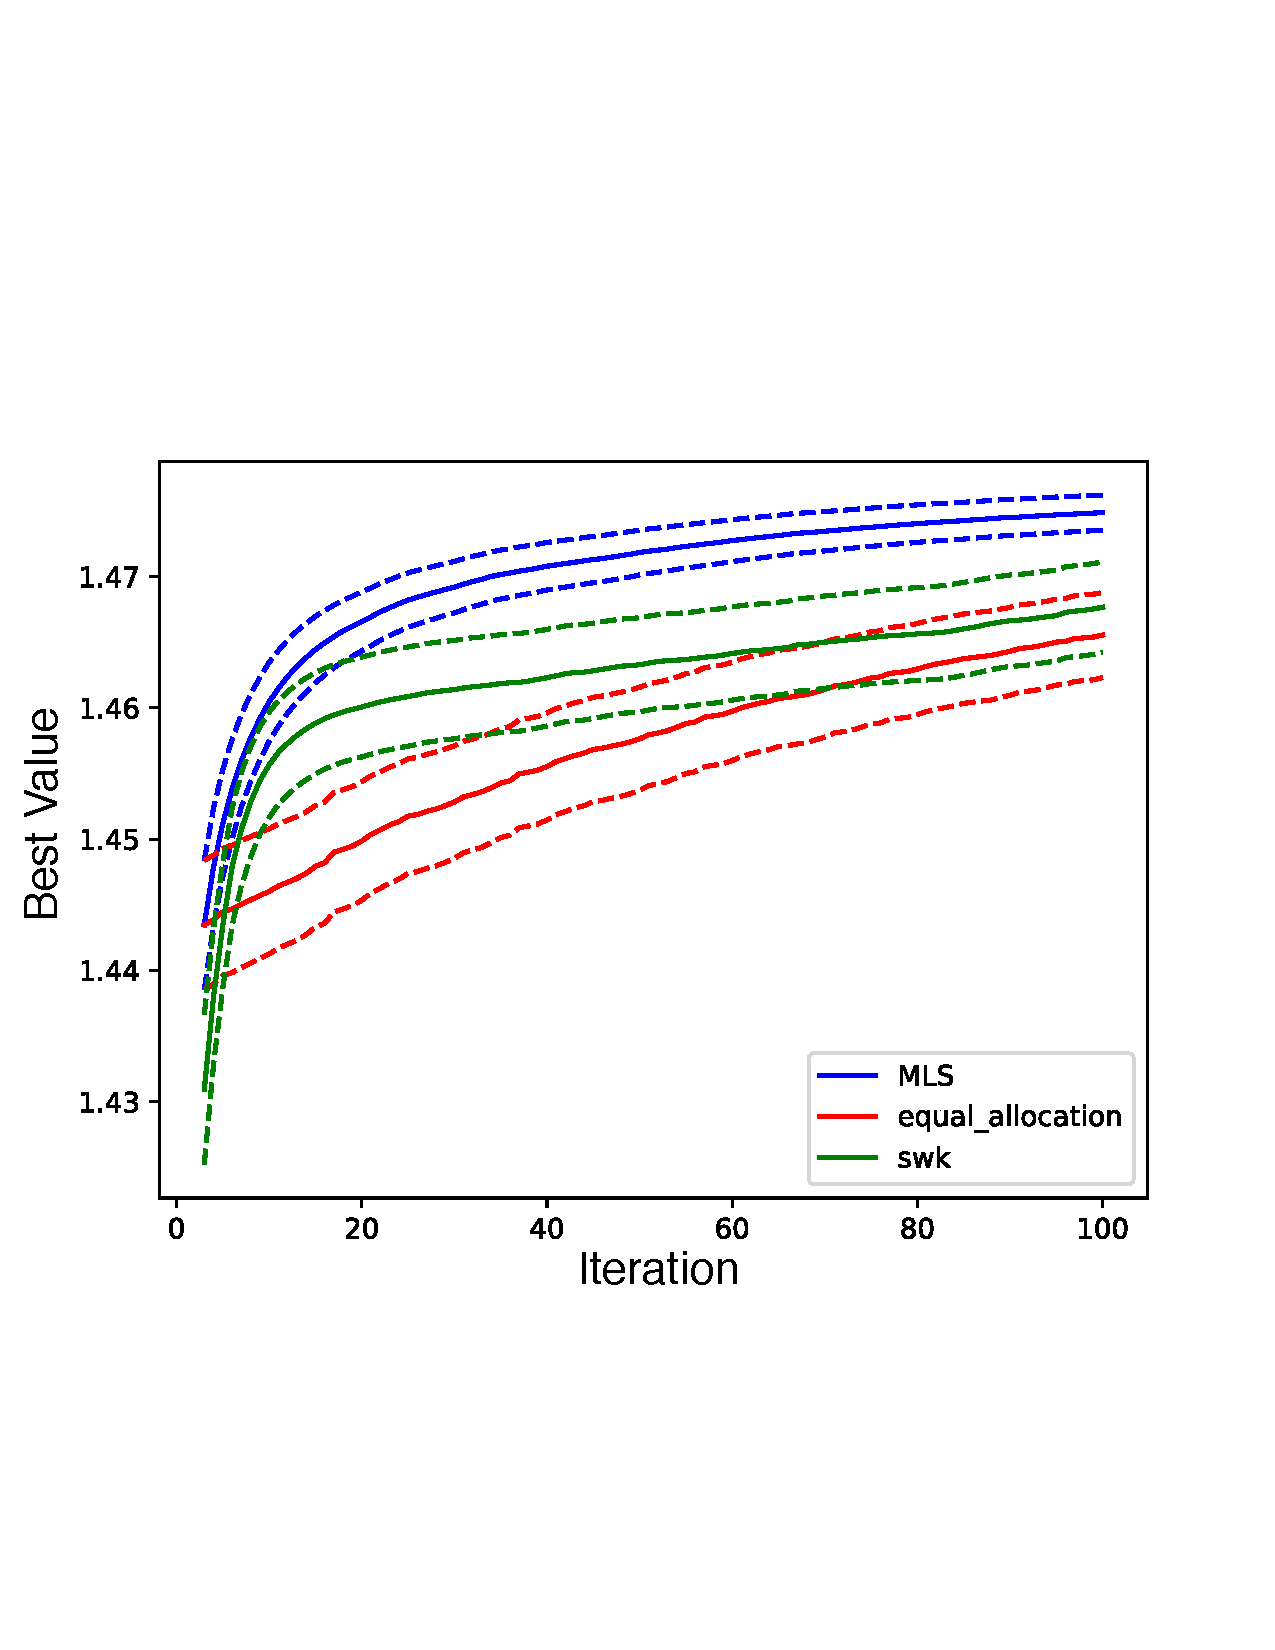
\includegraphics[width=0.32\linewidth,height=2.0in]{problem5_MLS_random__uniform_swk_best_solution.pdf}
}
\smallskip
\caption{
The SGD-GP statistical model (b) and \abbrv\ allocation rule (c) on the problem (a) from $\mathsection$\ref{local_maximum}. (b) shows that SGD-GP can predict the start's limiting objective value with high precision after 20 iterations. (c) shows that our policy does better than the other policies after only 8 iterations.
\label{fig:multiple_maxima}}
\end{center}
\end{figure}



\subsection{Objective Function with a Vanishing Gradient}
\label{gradient_vanishing}

Here we consider an objective function whose gradient is almost zero in a portion of the domain, $f(x):=(x+\sin{x})e^{-x^{2}}$, with a domain of $[-10,10]$. The stochastic gradient is equal to the true gradient plus normally distributed noise with mean 0 and variance 100.
Figure~\ref{fig:gradient_vanishing} compares the performance of \abbrv\ and equal allocation with $20$ starting points, plotting the number of iterations beyond the first stage on the $x$ axis, and the average maximum solution. We average over 1100 independent runs of \abbrv\ , equal allocation, and Swersky's statistical model with the MLS allocation rule. 

\stedit{Figure~\ref{fig:gradient_vanishing}.c shows that \abbrv\ performs much better than the other policies considered. Our policy performs better than the other policies after only 10 iterations, and it is significantly closer to the global optimum after 100 iterations than the other policies. The increasing trend of the curve of our policy indicates that it will find the global optimum after a few more iterations. Moreover, (b) shows that our statistical model predicts with very high precision a start's limiting objective value after 15 iterations. }


%\clearpage

\begin{figure}[htbp]
\begin{center}
\subcaptionbox{Objective function \\ $f(x):=(x+\sin{x})e^{-x^{2}}$}[0.32\linewidth]{
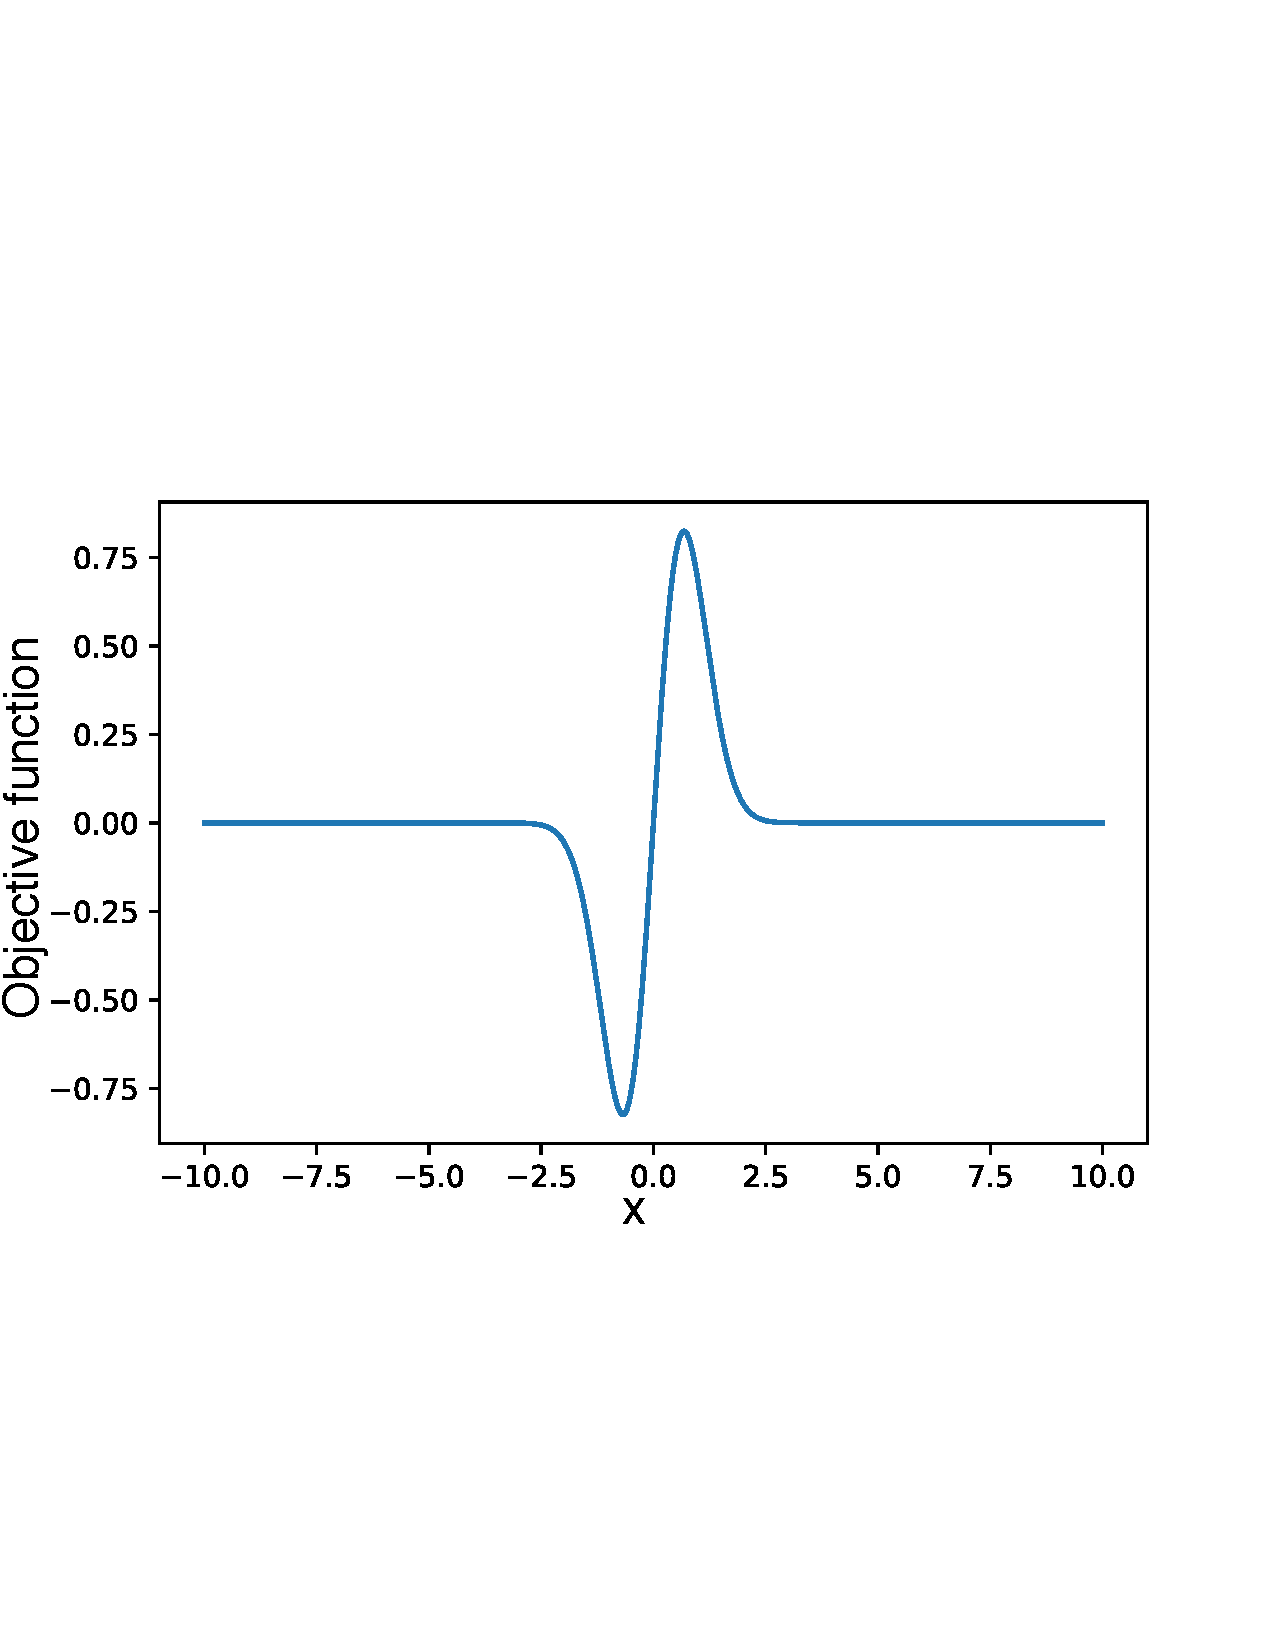
\includegraphics[width=0.32\linewidth,height=2.1in]{plot_problem6.pdf}}
%   \quad
\subcaptionbox{
SGD-GP's predictions and confidence intervals for the limiting value of SGD ($0.0$) from a single start.
}[0.32\linewidth]{
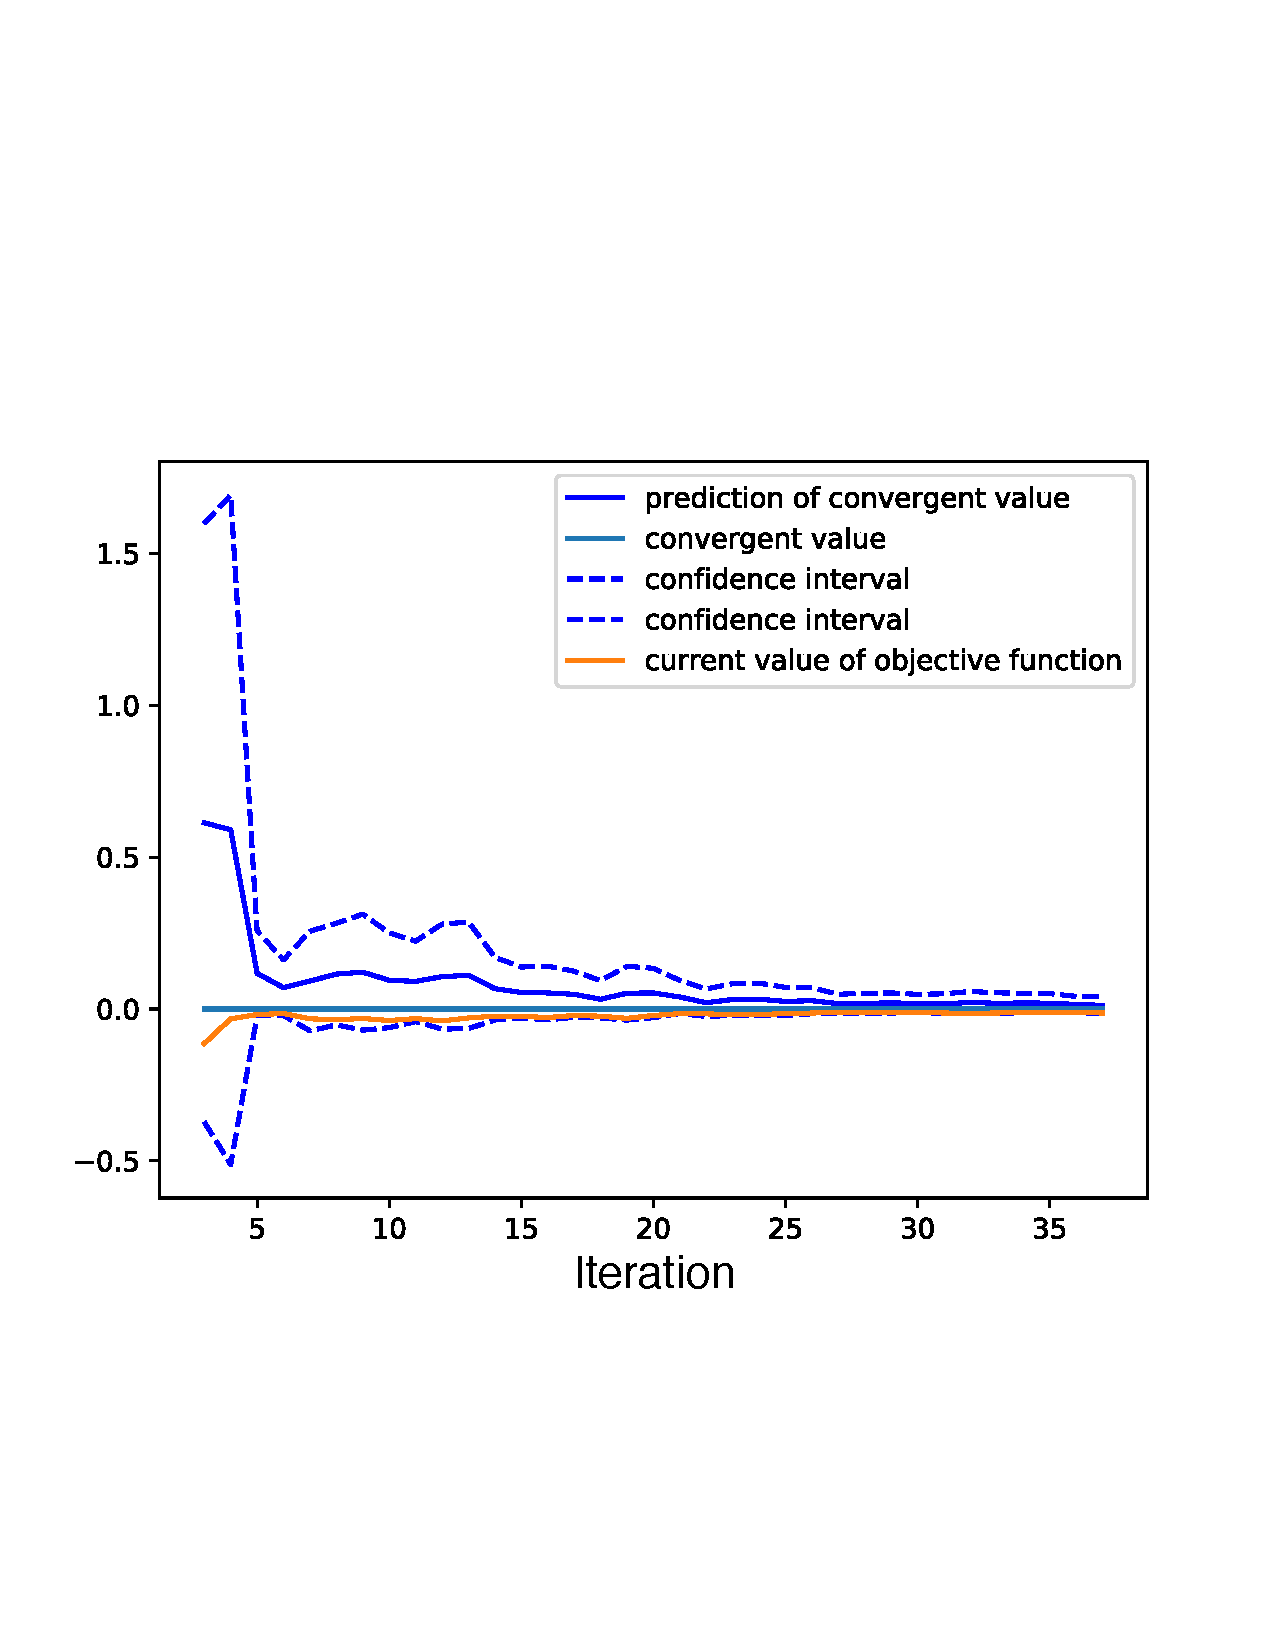
\includegraphics[width=0.32\linewidth,height=2.1in]{statistical_model_problem6.pdf}}
\quad
\subcaptionbox{
Performance comparison between \abbrv\, equal allocation, and Swersky's statistical model with the \abbrv\ rule using $20$ starting points.
}[0.32\linewidth]{
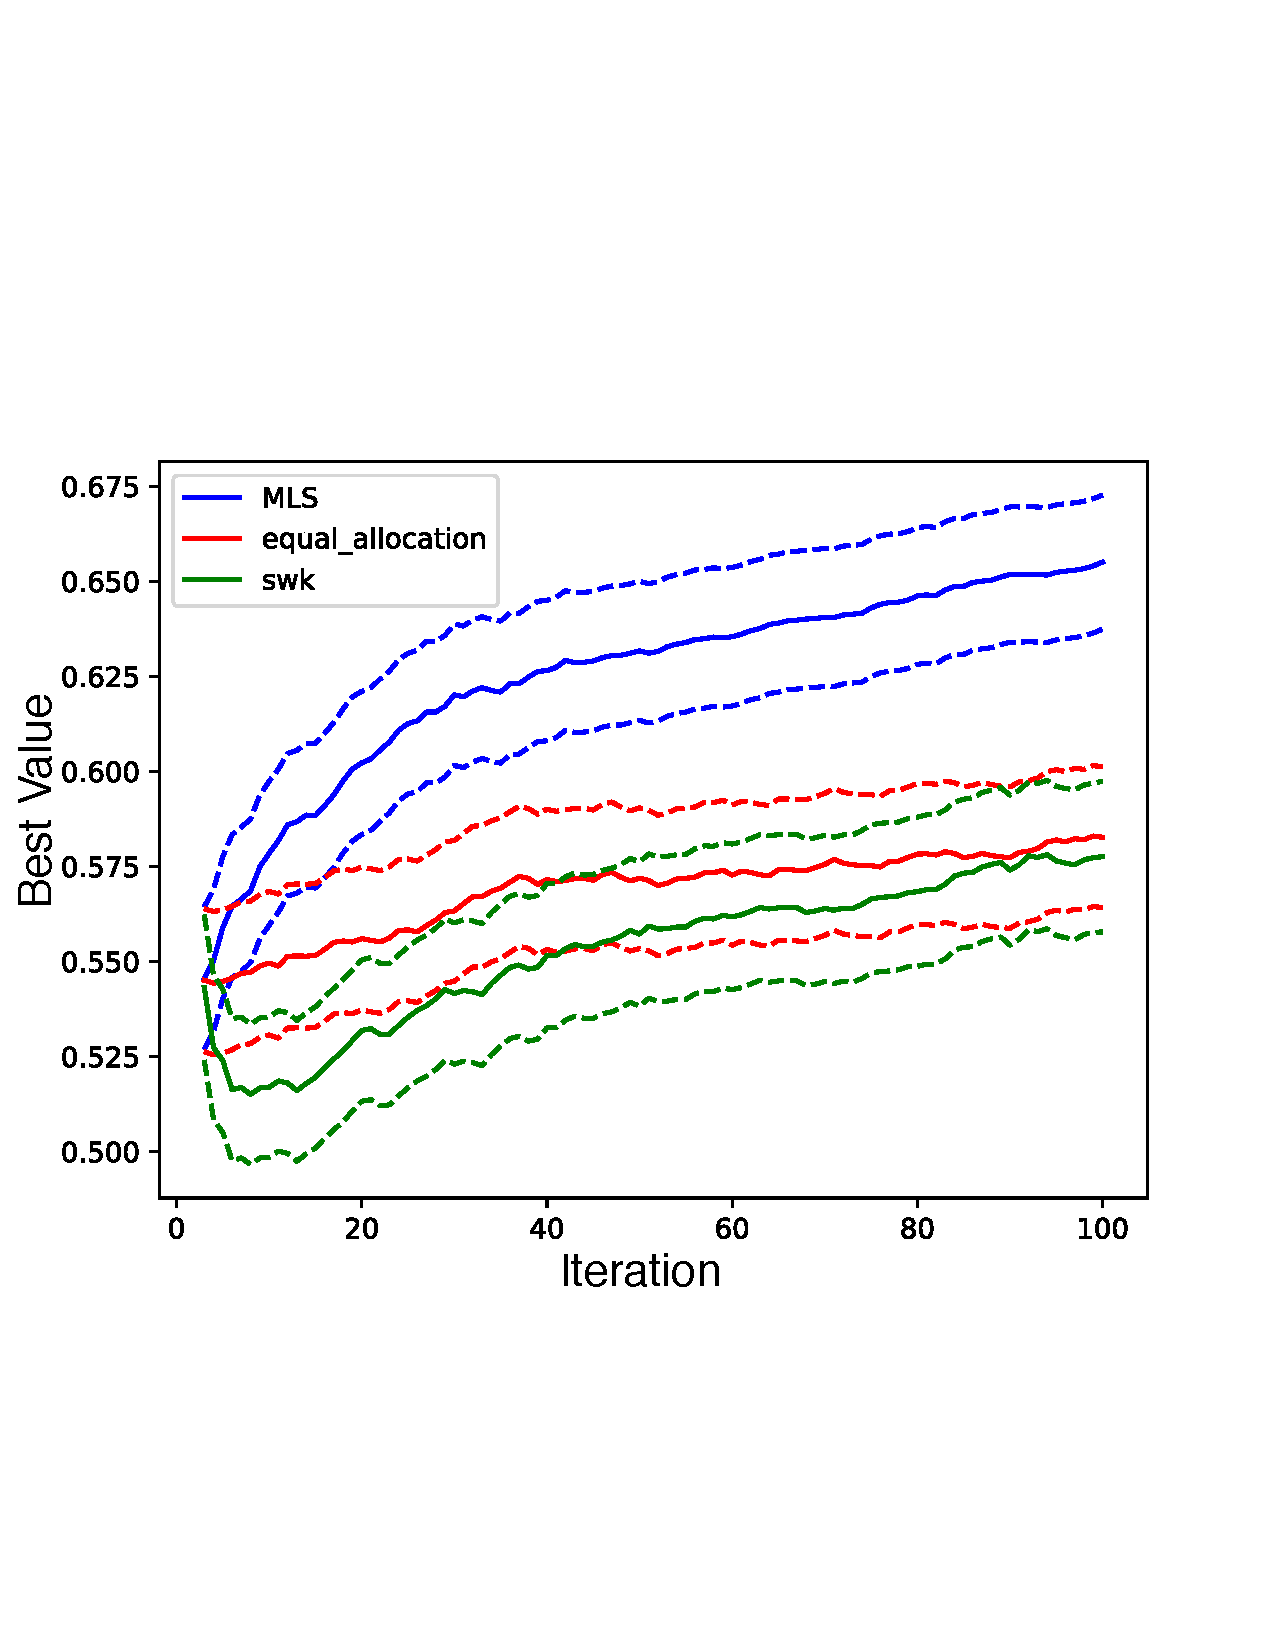
\includegraphics[width=0.32\linewidth,height=2.0in]{MLS_random__uniform_swk_best_solution.pdf}
}
\smallskip
\caption{
The SGD-GP statistical model (b) and \abbrv\ allocation rule (c) on the problem (a) from $\mathsection$\ref{gradient_vanishing}. (b) shows that SGD-GP can predict a start's limiting objective value with high precision after 15 iterations. (c) shows that our policy allocates resources to promising starters since the beginning, while the other policies waste resources moving not promising starters.\label{fig:gradient_vanishing}}
\end{center}
\end{figure}

\subsection{The 20-Dimensional Rosenbrock Function}
\label{rosenbrock}

Here we consider the 20-dimensional Rosenbrock function:

\[
f(x)=\sum_{i=1}^{19}\left[100\left(x_{i+1}-x_{i}^{2}\right)^{2}+\left(1-x_{i}\right)^{2}\right].
\]

We assume that we can only observe noisy evaluations of $f$: $y(x)=f(x)+\epsilon(x)$ where $\epsilon(x)\sim N(0, 0.1)$. The stochastic gradient is equal to the true gradient plus normally distributed noise with mean 0 and variance 0.1. We average over 1000 independent runs of \abbrv\, equal allocation, and random allocation using 30 starting points. 

\stedit{Figure~\ref{fig:rosenbrock} shows that \abbrv\ performs much better than the other policies considered. Our policy performs similar to the other policies when it is exploring the starters during the first 45 iterations, but then it finds a very good starter and it allocates most of the resources on that starter, and our solution starts to get much better. The equal allocation policy gets worse around iteration number 64 because each starter has been moved at most 2 steps, and the learning rate is still large and the gradients are stochastic. However, our policy is choosing a starter that has been moved more than 25 times, and the learning rate is low for that starter.}


%\clearpage

\begin{figure}[!htbp]
\begin{center}
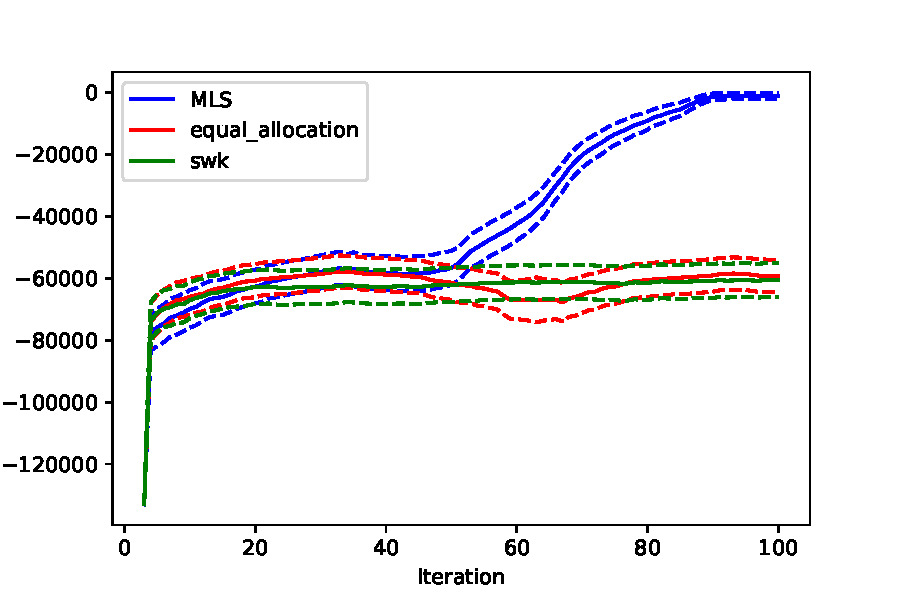
\includegraphics[width=0.50\linewidth]{new_plot.pdf}
\caption{
Performance comparison between \abbrv\, equal allocation, and random allocation using $30$ starting points. Our policy does much better than the other policies after only 45 iterations. In fact, after only 100 iterations, our policy finds the global optimum, while the other policies are very far away from a good solution. This problem shows that our policy works extremely well on high-dimensional problems where the objective function is noisy.
\label{fig:rosenbrock}}
\end{center}
\end{figure}







%\subsection{Comparison of SGD-GP to a Statistical Model with Exact Gradients}
%We also compare the accuracy of the approximations SGD-GP to an alternate statistical model that can be constructed using exact gradients, and that %avoids the approximations SGD-GP makes in section~\ref{sec:SGD-GP-2}.

%Recall that Section~\ref{sec:SGD-GP-2} performed inference over $f(x_\infty)$ using the mean value theorem, the relationship $f\left(x_{\infty}\right)=f\left(x_{n}\right)+L_{n}\left|x_{\infty}-x_{n}\right|$, and an estimate of $L_n$ based on approximations.
%Another method we considered was to use Taylor's theorem to write,
%\[
%f\left(x_{\infty}\right)\approx f\left(x_{n}\right)-\nabla f\left(x_{n}\right)\frac{M_{n}}{\sqrt{n}}.
%\]
%Then, if we had access to exact observations of $f(x_\infty)$ or could estimate it with high precision based on repeated simulation after each batch, then we could use this relationship together with our posterior on $M(n)$ to construct a posterior on $f(x_\infty)$.

%Figure~\ref{fig:SGD-GP} compares the posterior distributions created by the two methods on the problem from Sections~\ref{concave}, where SGD-GP has access only to stochastic gradients, and this alternate method sees exact gradients.  We see that the inference performed by the two methods is similar.

%\begin{figure}[tb]
%\centering
%\subcaptionbox{SGD-GP}[0.32\linewidth]{
%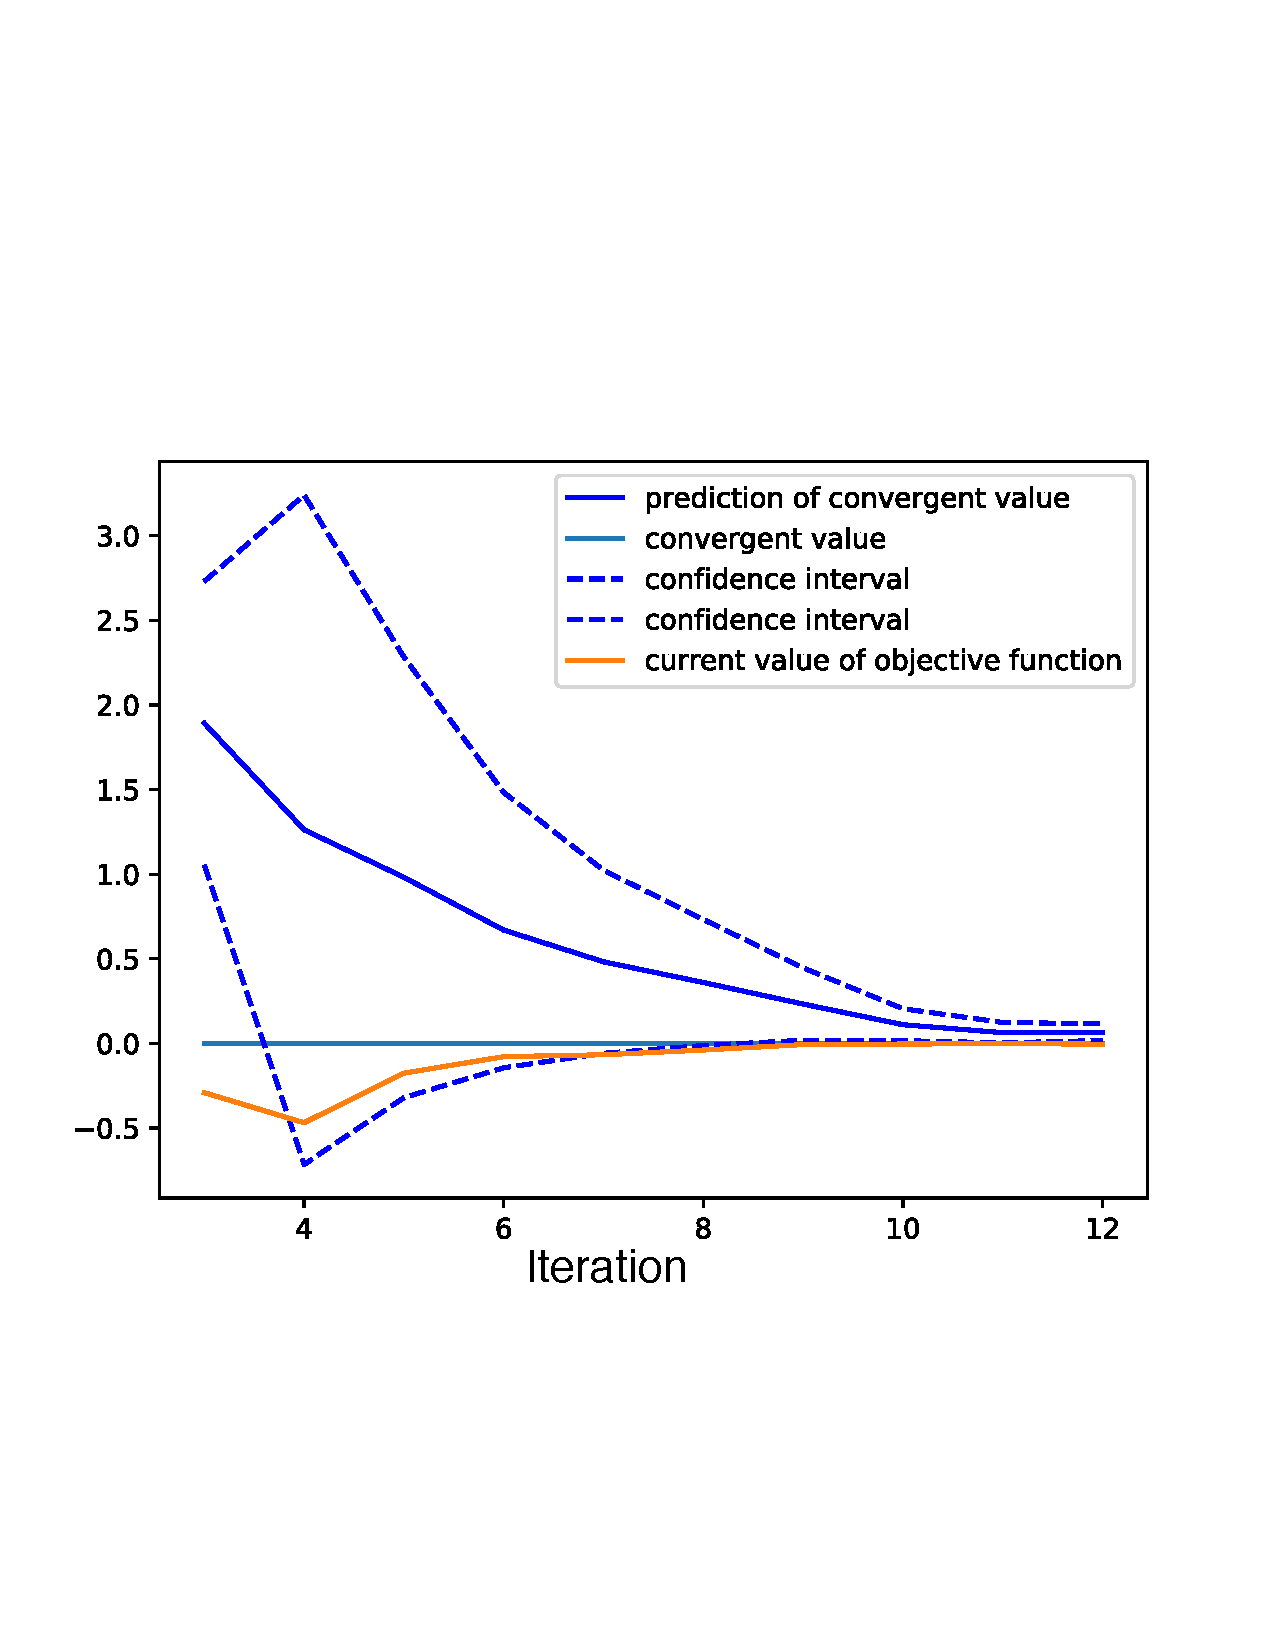
\includegraphics[width=0.32\linewidth,height=2.1in]{quadratic_stat_approx_lipschitz.pdf}}
%\subcaptionbox{Alternative statistical method with exact gradients}[0.32\linewidth]{
%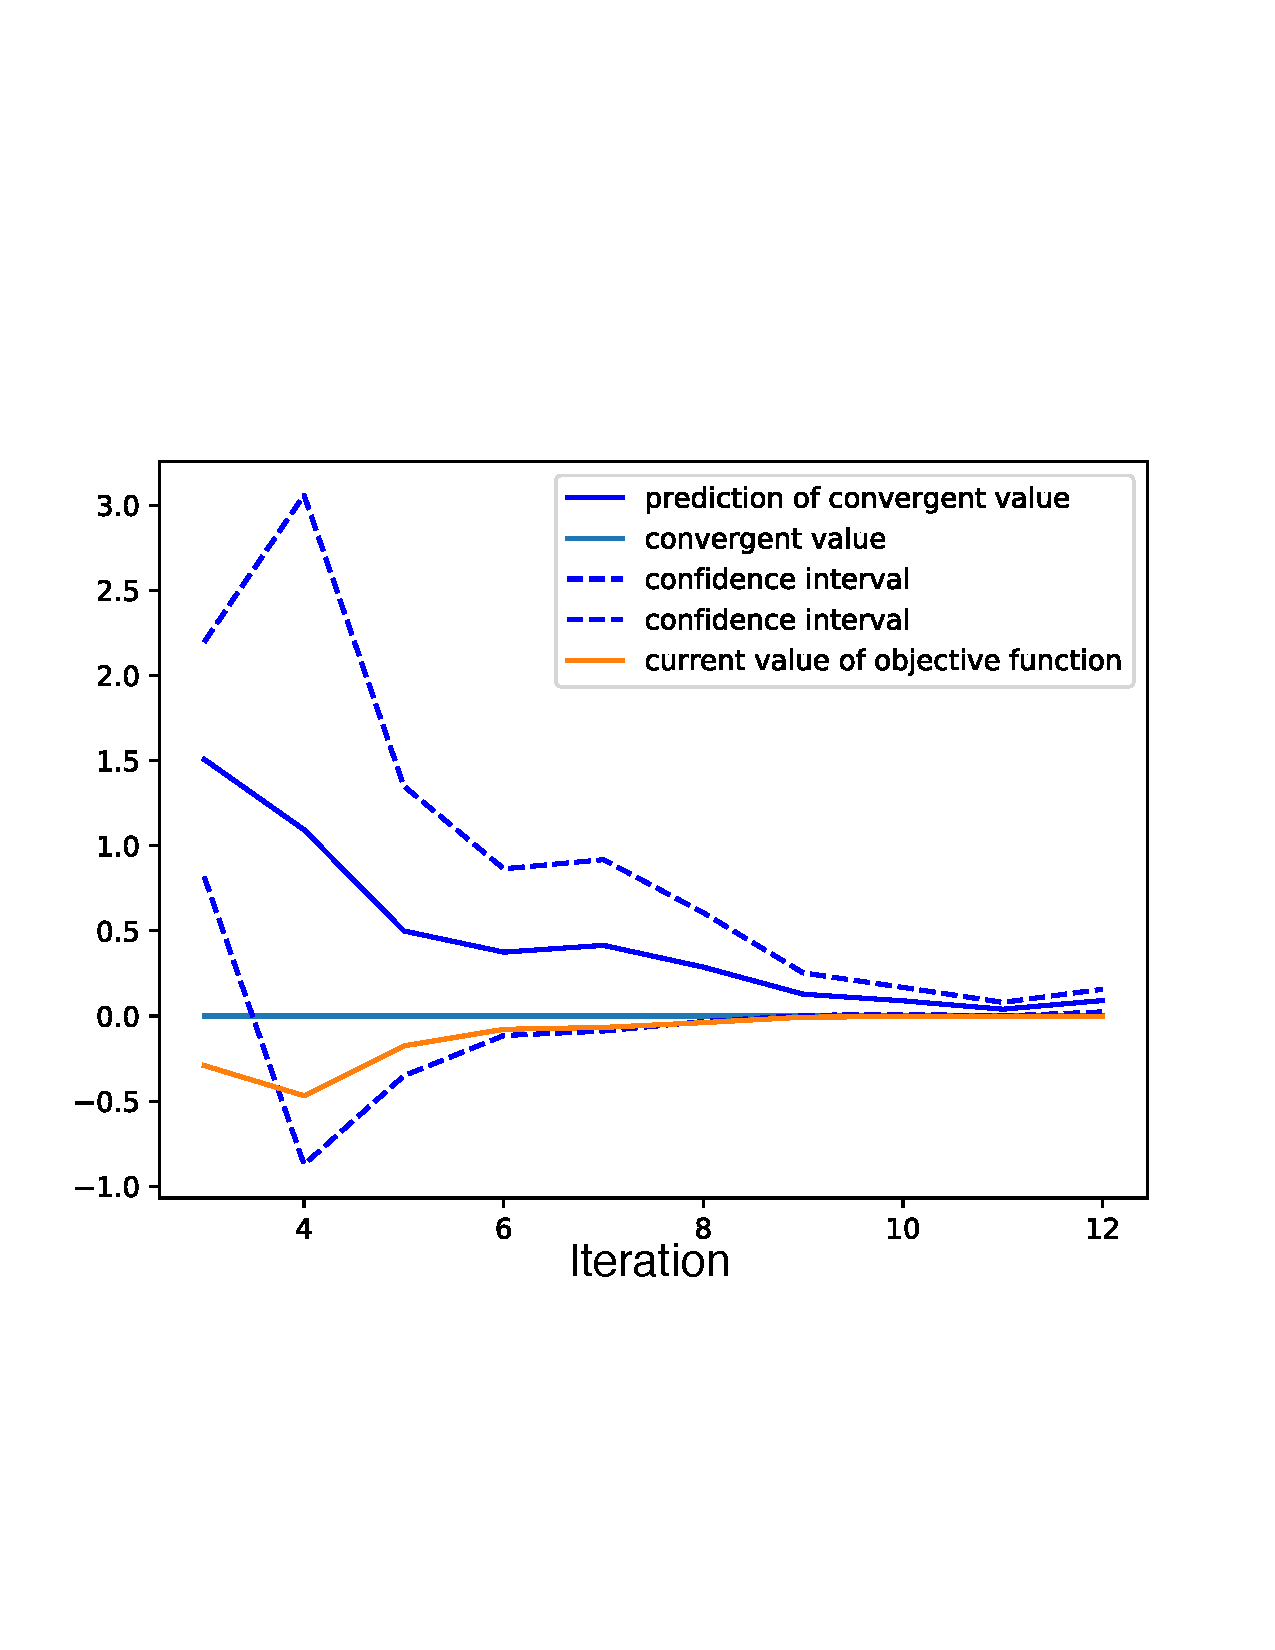
\includegraphics[width=0.32\linewidth,height=2.1in]{real_gradient_stat.pdf}}
%\caption{Comparison between SGD-GP and an alternate statistical model that assumes exact gradient observations and avoids the approximations SGD-GP uses in Sections~\ref{sec:SGD-GP-2}.  Data is generated from the quadratic problem from $\mathsection$\ref{concave}. The predictions and confidence intervals from the two methods are similar.}
%\label{fig:SGD-GP}
%\end{figure}



\section{CONCLUSION}
\label{conclusion}

We presented \name\ (\abbrv), which is a new allocation rule across starts that decreases computational effort when using multi-start stochastic gradient ascent to globally optimize a function. \abbrv\ depends on a new non-parametric statistical model, which is derived from the asymptotic theory of stochastic gradient ascent. It outperforms two benchmarks in numerical experiments.
 
\section*{ACKNOWLEDGMENTS}
The authors were partially supported by NSF CAREER CMMI-1254298, NSF CMMI-1536895, and AFOSR FA9550-15-1-0038.






\appendix

\section*{Appendix}
%\label{appendix}

%\renewcommand{\thesubsection}{\Alph{subsection}}

\section{APPENDICES} 
\label{app:THEOREMS}

In this section we state two theorems from \cite{kushner} about limit theory of SGD algorithms. The first theorem shows the existence of limit points of SGD algorithms. The second theorem shows that if convergence occurs, the normalized sequence of points of SGD $M_{n}:=\sqrt{n}\left(x_{n}-x_{\infty}\right)$ converges weakly to a known stochastic process, which is a Ornstein-Uhlenbeck process under some assumptions. 

\begin{theorem} 
(Theorem 2.1 of Section 5.2 of \cite{kushner}) 
Suppose that the learning rates $\left\{ \lambda_{n}\right\}$ of the stochastic gradient descent satisfy that $\sum_{n=1}^{\infty}\lambda_{n}=\infty$, $\lambda_{n}\geq0$, $\lambda_{n}\rightarrow0$ and $\sum_{n=1}^{\infty}\lambda_{n}^{2}<\infty$. In addition, suppose the following

\begin{enumerate}
\item $\mbox{sup}_{n}E\left[\left|Y_{n}\right|^{2}\right]<\infty$.
\item There is a measurable and continuous function $g$ and random variables $\beta_{n}$ such that 
\[
E_{n}Y_{n}=E\left[Y_{n}\mid x_{1},Y_{i},i<n\right]=g\left(x_{n}\right)+\beta_{n},
\]
and $\sum_{i}\lambda_{i}\left|\beta_{i}\right|<\infty \mbox{ a.s.}$
\end{enumerate}

Then 
$\left\{ x_{n}\right\} $ converges to some limit set of the ODE $\overset{\cdot}{x}=g\left(x\right)$ in $A$ (see section 5.2 of \cite{kushner}). If the objective function $f$ is continuously differentiable, $g=-\nabla f$, and $f$ is constant on each of the disjoint compact and connected subsets $S_{j}$ of the stationary points, then $x_{n}$ converges almost surely to a unique $S_{i}$.
\end{theorem}

\begin{theorem} 
(Theorem 2.1 of section 10.2.1 of \cite{kushner}) 
Let $x_{\infty}$ be a limit point in the interior of $A$. Suppose that there is a measurable and continuous function $g$ such that $E_{n}Y_{n}=E\left[Y_{n}\mid x_{1},Y_{i},i<n\right]=g\left(x_{n}\right)$. In addition, assume that 

\begin{enumerate}
\item $\lambda_{n}:=1/n$.
\item $\left\{ Y_{n}1_{\{\left|x_{n}-x_{\infty}\right|\}\leq\rho}\right\}$ is uniformly integrable for small $\rho$.
\item $M_{n}:=\left(\frac{x_{n}-x_{\infty}}{\sqrt{\epsilon_{n}}}\right)$ is tight.
\item $E_{n}Y_{n}=g_{n}\left(x_{n}\right)$, where $g_{n}$ is continuously differentiable for each $n$, and $g_{n}\left(x\right)=g_{n}\left(x_{\infty}\right)+g'_{n,x}\left(x_{\infty}\right)\left(x-x_{\infty}\right)+o\left(\left|x-x_{\infty}\right|\right)$.
\item $\lim_{n,m}\frac{1}{\sqrt{m}}\sum_{i=n}^{n+mt-1}g_{i}\left(x_{\infty}\right)=0$, where the limit is uniform in some bounded t-interval.
\item There is a Hurwitz matrix $Q$ (i.e., the real parts of the eigenvalues of $Q$ are negative) such that 
\[
\lim_{n,m}\frac{1}{m}\sum_{i=n}^{n+m-1}\left[g'_{i,x}\left(x_{\infty}\right)-Q\right]=0, 
\]
and $Q+I/2$ is also a Hurwitz matrix.
\item For some $p>0$ and small $\rho>0$, $\sup_{n}E\left|\delta R_{n}\right|^{2+p}1_{\left\{ \left|x_{n}-x_{\infty}\right|\leq\rho\right\} }<\infty$, where $\delta R_{n}=Y_{n}-E\left[Y_{n}\mid x_{1},Y_{i},i<n\right]$.
\end{enumerate}

We then have that the process $M^{n}\left(t\right):=\frac{\left(x_{n+i}-x_{\infty}\right)}{\sqrt{\epsilon_{n+i}}}$ if $t\in \left[i,i+1\right]$, converges weakly to 
\[
M\left(t\right):=\int_{-\infty}^{t}e^{\left(Q+I/2\right)\left(t-s\right)}dW\left(s\right)
\]
where $W$ is a Wiener process with some covariance matrix $\Sigma_{1}$.
\end{theorem}

In the previous theorem, the limit of the process $M^{n}\left(t\right)$ is defined by the SDE $dM(t)=(Q+I/2)M(t)dt+dW(t)$, and so $M$ is an Ornstein-Uhlenbeck process when the domain is an interval in $\mathbb{R}$, because $Q+I/2$ is negative in this case.

\bibliographystyle{wsc}
\bibliography{or}


%%%%%%%%%%%%%%%%%
\end{document}
%%%%%%%%%%%%%%%%%





